% Options for packages loaded elsewhere
\PassOptionsToPackage{unicode}{hyperref}
\PassOptionsToPackage{hyphens}{url}
%
\documentclass[
]{book}
\usepackage{lmodern}
\usepackage{amsmath}
\usepackage{ifxetex,ifluatex}
\ifnum 0\ifxetex 1\fi\ifluatex 1\fi=0 % if pdftex
  \usepackage[T1]{fontenc}
  \usepackage[utf8]{inputenc}
  \usepackage{textcomp} % provide euro and other symbols
  \usepackage{amssymb}
\else % if luatex or xetex
  \usepackage{unicode-math}
  \defaultfontfeatures{Scale=MatchLowercase}
  \defaultfontfeatures[\rmfamily]{Ligatures=TeX,Scale=1}
\fi
% Use upquote if available, for straight quotes in verbatim environments
\IfFileExists{upquote.sty}{\usepackage{upquote}}{}
\IfFileExists{microtype.sty}{% use microtype if available
  \usepackage[]{microtype}
  \UseMicrotypeSet[protrusion]{basicmath} % disable protrusion for tt fonts
}{}
\makeatletter
\@ifundefined{KOMAClassName}{% if non-KOMA class
  \IfFileExists{parskip.sty}{%
    \usepackage{parskip}
  }{% else
    \setlength{\parindent}{0pt}
    \setlength{\parskip}{6pt plus 2pt minus 1pt}}
}{% if KOMA class
  \KOMAoptions{parskip=half}}
\makeatother
\usepackage{xcolor}
\IfFileExists{xurl.sty}{\usepackage{xurl}}{} % add URL line breaks if available
\IfFileExists{bookmark.sty}{\usepackage{bookmark}}{\usepackage{hyperref}}
\hypersetup{
  pdftitle={EDS 221: SCIENTIFIC PROGRAMMING ESSENTIALS},
  pdfauthor={Allison Horst},
  hidelinks,
  pdfcreator={LaTeX via pandoc}}
\urlstyle{same} % disable monospaced font for URLs
\usepackage{color}
\usepackage{fancyvrb}
\newcommand{\VerbBar}{|}
\newcommand{\VERB}{\Verb[commandchars=\\\{\}]}
\DefineVerbatimEnvironment{Highlighting}{Verbatim}{commandchars=\\\{\}}
% Add ',fontsize=\small' for more characters per line
\usepackage{framed}
\definecolor{shadecolor}{RGB}{248,248,248}
\newenvironment{Shaded}{\begin{snugshade}}{\end{snugshade}}
\newcommand{\AlertTok}[1]{\textcolor[rgb]{0.94,0.16,0.16}{#1}}
\newcommand{\AnnotationTok}[1]{\textcolor[rgb]{0.56,0.35,0.01}{\textbf{\textit{#1}}}}
\newcommand{\AttributeTok}[1]{\textcolor[rgb]{0.77,0.63,0.00}{#1}}
\newcommand{\BaseNTok}[1]{\textcolor[rgb]{0.00,0.00,0.81}{#1}}
\newcommand{\BuiltInTok}[1]{#1}
\newcommand{\CharTok}[1]{\textcolor[rgb]{0.31,0.60,0.02}{#1}}
\newcommand{\CommentTok}[1]{\textcolor[rgb]{0.56,0.35,0.01}{\textit{#1}}}
\newcommand{\CommentVarTok}[1]{\textcolor[rgb]{0.56,0.35,0.01}{\textbf{\textit{#1}}}}
\newcommand{\ConstantTok}[1]{\textcolor[rgb]{0.00,0.00,0.00}{#1}}
\newcommand{\ControlFlowTok}[1]{\textcolor[rgb]{0.13,0.29,0.53}{\textbf{#1}}}
\newcommand{\DataTypeTok}[1]{\textcolor[rgb]{0.13,0.29,0.53}{#1}}
\newcommand{\DecValTok}[1]{\textcolor[rgb]{0.00,0.00,0.81}{#1}}
\newcommand{\DocumentationTok}[1]{\textcolor[rgb]{0.56,0.35,0.01}{\textbf{\textit{#1}}}}
\newcommand{\ErrorTok}[1]{\textcolor[rgb]{0.64,0.00,0.00}{\textbf{#1}}}
\newcommand{\ExtensionTok}[1]{#1}
\newcommand{\FloatTok}[1]{\textcolor[rgb]{0.00,0.00,0.81}{#1}}
\newcommand{\FunctionTok}[1]{\textcolor[rgb]{0.00,0.00,0.00}{#1}}
\newcommand{\ImportTok}[1]{#1}
\newcommand{\InformationTok}[1]{\textcolor[rgb]{0.56,0.35,0.01}{\textbf{\textit{#1}}}}
\newcommand{\KeywordTok}[1]{\textcolor[rgb]{0.13,0.29,0.53}{\textbf{#1}}}
\newcommand{\NormalTok}[1]{#1}
\newcommand{\OperatorTok}[1]{\textcolor[rgb]{0.81,0.36,0.00}{\textbf{#1}}}
\newcommand{\OtherTok}[1]{\textcolor[rgb]{0.56,0.35,0.01}{#1}}
\newcommand{\PreprocessorTok}[1]{\textcolor[rgb]{0.56,0.35,0.01}{\textit{#1}}}
\newcommand{\RegionMarkerTok}[1]{#1}
\newcommand{\SpecialCharTok}[1]{\textcolor[rgb]{0.00,0.00,0.00}{#1}}
\newcommand{\SpecialStringTok}[1]{\textcolor[rgb]{0.31,0.60,0.02}{#1}}
\newcommand{\StringTok}[1]{\textcolor[rgb]{0.31,0.60,0.02}{#1}}
\newcommand{\VariableTok}[1]{\textcolor[rgb]{0.00,0.00,0.00}{#1}}
\newcommand{\VerbatimStringTok}[1]{\textcolor[rgb]{0.31,0.60,0.02}{#1}}
\newcommand{\WarningTok}[1]{\textcolor[rgb]{0.56,0.35,0.01}{\textbf{\textit{#1}}}}
\usepackage{longtable,booktabs}
\usepackage{calc} % for calculating minipage widths
% Correct order of tables after \paragraph or \subparagraph
\usepackage{etoolbox}
\makeatletter
\patchcmd\longtable{\par}{\if@noskipsec\mbox{}\fi\par}{}{}
\makeatother
% Allow footnotes in longtable head/foot
\IfFileExists{footnotehyper.sty}{\usepackage{footnotehyper}}{\usepackage{footnote}}
\makesavenoteenv{longtable}
\usepackage{graphicx}
\makeatletter
\def\maxwidth{\ifdim\Gin@nat@width>\linewidth\linewidth\else\Gin@nat@width\fi}
\def\maxheight{\ifdim\Gin@nat@height>\textheight\textheight\else\Gin@nat@height\fi}
\makeatother
% Scale images if necessary, so that they will not overflow the page
% margins by default, and it is still possible to overwrite the defaults
% using explicit options in \includegraphics[width, height, ...]{}
\setkeys{Gin}{width=\maxwidth,height=\maxheight,keepaspectratio}
% Set default figure placement to htbp
\makeatletter
\def\fps@figure{htbp}
\makeatother
\setlength{\emergencystretch}{3em} % prevent overfull lines
\providecommand{\tightlist}{%
  \setlength{\itemsep}{0pt}\setlength{\parskip}{0pt}}
\setcounter{secnumdepth}{5}
\usepackage{booktabs}
\usepackage{booktabs}
\usepackage{longtable}
\usepackage{array}
\usepackage{multirow}
\usepackage{wrapfig}
\usepackage{float}
\usepackage{colortbl}
\usepackage{pdflscape}
\usepackage{tabu}
\usepackage{threeparttable}
\usepackage{threeparttablex}
\usepackage[normalem]{ulem}
\usepackage{makecell}
\usepackage{xcolor}
\ifluatex
  \usepackage{selnolig}  % disable illegal ligatures
\fi
\usepackage[]{natbib}
\bibliographystyle{apalike}

\title{EDS 221: SCIENTIFIC PROGRAMMING ESSENTIALS}
\author{Allison Horst}
\date{}

\begin{document}
\maketitle

{
\setcounter{tocdepth}{1}
\tableofcontents
}
\hypertarget{scientific-programming-essentials-for-environmental-data-science}{%
\chapter{Scientific programming essentials for environmental data science}\label{scientific-programming-essentials-for-environmental-data-science}}

\hypertarget{material-disclaimer-and-use}{%
\subsection*{Material disclaimer and use}\label{material-disclaimer-and-use}}
\addcontentsline{toc}{subsection}{Material disclaimer and use}

This book was created by \href{www.allisonhorst.com}{Allison Horst} for EDS 221 (Scientific Programming Essentials) in the Bren School's 1-year \href{https://bren.ucsb.edu/masters-programs/master-environmental-data-science}{Master of Environmental Data Science program} at UC Santa Barbara. It accompanies lecture, computational lab and discussion materials that may or may not be linked to throughout the book. This book is intended as a supplemental resource for some parts of the course. In other words, it is not intended as a standalone textbook.

All materials in this book are openly available for use and reuse by Creative Commons Attribution and Share-Alike license.

\href{https://creativecommons.org/licenses/}{
\includegraphics[width=1.29167in,height=\textheight]{images/cc_by_sa.png}}

Thank you in advance for suggestions and corrections, which can be submitted as issue to this \href{https://github.com/allisonhorst/eds-221}{GitHub repo}.

\hypertarget{acknowledgments}{%
\subsection*{Acknowledgments}\label{acknowledgments}}
\addcontentsline{toc}{subsection}{Acknowledgments}

I create my courses while standing on shoulders of generous teaching and developing giants in R, data science, and education communities. The wealth and quality of open educational resources (OERs) in data science has made teaching in the field fun, innovative, and inspiring. I've tried to thoroughly credit authors resources that I have pulled from and adapted for this book, and I welcome additions if I have missed any that should be included.

\hypertarget{course-introduction}{%
\section{Course introduction}\label{course-introduction}}

\begin{figure}

{\centering 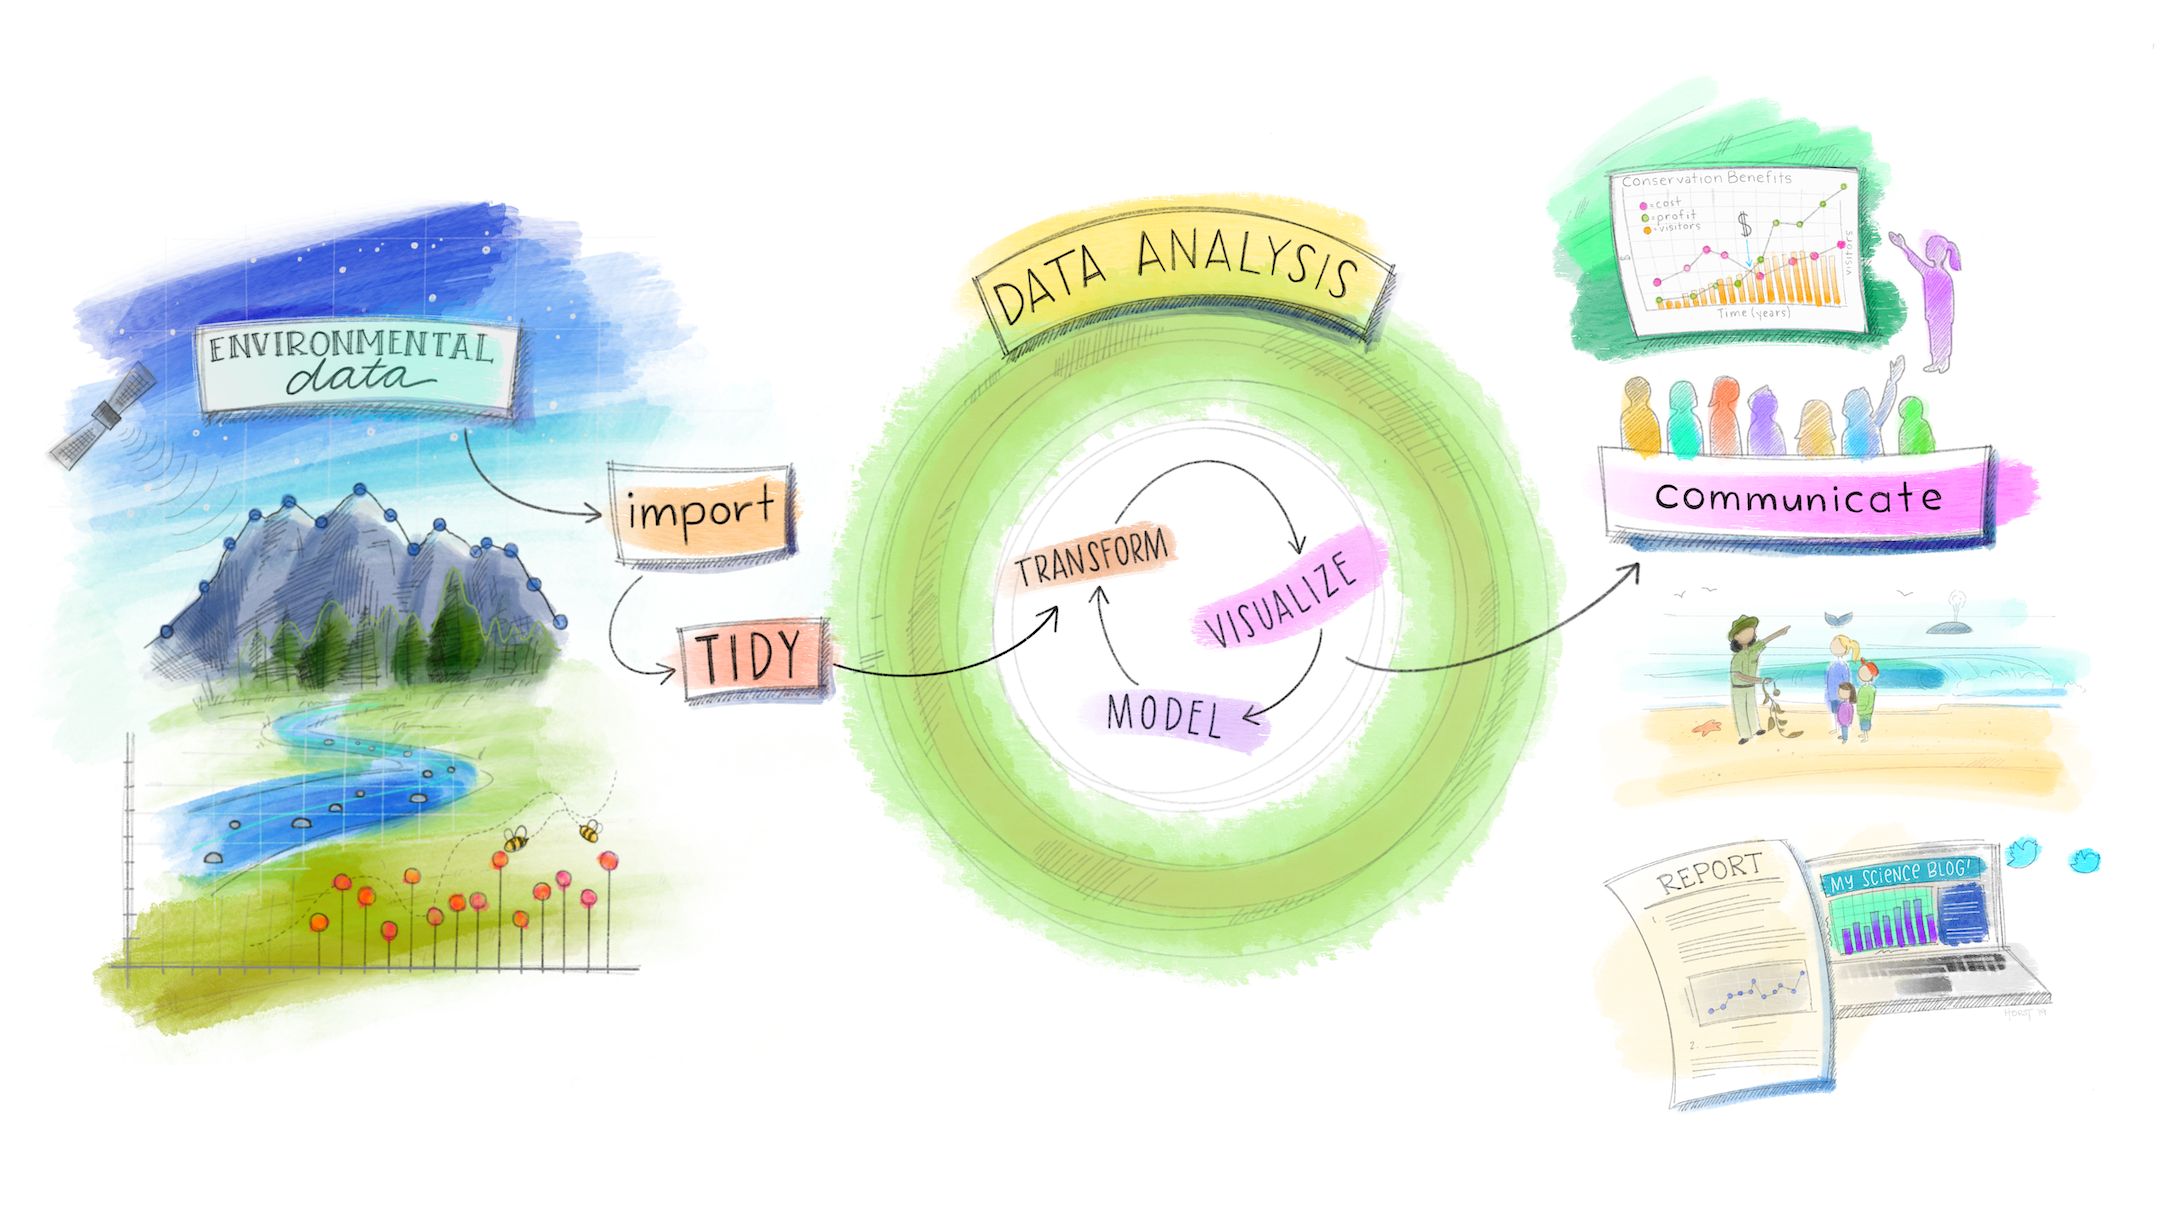
\includegraphics[width=1\linewidth]{images/eds_r4ds} 

}

\caption{Slide from Dr. Julia Lowndes' 2019 keynote talk at useR conference (illustration by Allison Horst).}\label{fig:unnamed-chunk-1}
\end{figure}

As nicely summarized in the title of a \href{https://www.nceas.ucsb.edu/news/next-generation-environmental-scientists-are-data-scientists}{2018 NCEAS post}, \textbf{``the next generation of environmental scientists are data scientists''}. Over the next year in MEDS you'll build skills to responsibly apply advanced methods in environmental modeling, spatial data analysis, machine learning, and more to investigate, analyze and communicate with complex environmental data.

To get there, you'll need a strong foundation in programming basics like: understanding types and structures of data, basic data wrangling and visualization, algorithm development with functions, loops, and conditionals, and how to troubleshoot. While working in the weeds of programming, we'll also learn and reinforce transferable habits for reproducible workflows, robust file paths, version control, data organization, project management, and more.

In EDS 221 you'll also start building versatility by learning fundamental programming skills in different languages (R, Python) and integrated development environments (IDEs) like RStudio and PyCharm, while documenting our work in R Markdown and Jupyter Notebooks.

Upon the building blocks established in EDS 221, you'll be prepared to incrementally grow your advanced environmental data science toolkit throughout MEDS, then enter the workplace at the leading edge of quantitative methods in the field.

\hypertarget{links-to-course-materials}{%
\section{Links to course materials}\label{links-to-course-materials}}

\begin{itemize}
\tightlist
\item
  \href{https://docs.google.com/document/d/1OGbc6U3STKdsThUKd9Nj5UgzeB7djgM130ku1UUH1gU/edit?usp=sharing}{EDS 221 Syllabus}
\item
  Code of Conduct
\item
  EDS 221 GitHub site
\end{itemize}

\hypertarget{course-setup}{%
\section{Course setup}\label{course-setup}}

We will use the following in EDS 221. You should have pre-installed recent versions before starting the course.

\begin{itemize}
\tightlist
\item
  \href{https://www.r-project.org/}{R (Version 4.0.2 ``Taking Off Again'', or higher)}
\item
  \href{https://rstudio.com/products/rstudio/}{RStudio Desktop (version 1.4.1103 ``Wax Begonia'', or higher)}
\item
  \href{https://rstudio.cloud/}{RStudio Cloud account}
\item
  Python (version XXXXX or higher)
\item
  Pycharm (version XXXX or higher)
\end{itemize}

\hypertarget{course-resources}{%
\section{Course resources}\label{course-resources}}

\begin{itemize}
\item
  \href{https://rstudio-education.github.io/hopr/}{Hands-on Programming with R} by Garrett Grolemund
\item
  \href{https://r4ds.had.co.nz/}{R for Data Science} by Garrett Grolemund and Hadley Wickham
\item
  \href{https://adv-r.hadley.nz/}{Advanced R} by Hadley Wickham
\item
  \href{https://learnpythonbreakpython.com/}{Learn Python Break Python} by Scott Grant
\end{itemize}

\hypertarget{r-py}{%
\chapter{Meet the 221 tools}\label{r-py}}

\hypertarget{r}{%
\section{R}\label{r}}

\hypertarget{rstudio}{%
\section{RStudio}\label{rstudio}}

\hypertarget{python}{%
\section{Python}\label{python}}

\hypertarget{jupyter-notebooks}{%
\section{Jupyter Notebooks}\label{jupyter-notebooks}}

\hypertarget{types}{%
\chapter{Data structures and types}\label{types}}

How we work with data is largely dependent on the \emph{type} and \emph{structure} of data we're working with. That's more than just ``is this a number or letters?'' We need to understand how the data are stored so that we know how to access pieces of it, how our code will understand and interact with data, and so we're correctly predicting how data will change based on what we do with it.

In this chapter, we'll learn about different structures of data, and the types of data they can contain.

\hypertarget{data-structures}{%
\section{Data structures}\label{data-structures}}

\hypertarget{vectors}{%
\subsection{Vectors}\label{vectors}}

\hypertarget{tibbles}{%
\subsection{Tibbles}\label{tibbles}}

\hypertarget{matrices}{%
\subsection{Matrices}\label{matrices}}

\hypertarget{lists}{%
\subsection{Lists}\label{lists}}

\hypertarget{data-types}{%
\section{Data types}\label{data-types}}

See: \url{https://r4ds.had.co.nz/vectors.html}

\hypertarget{tidydata}{%
\chapter{Tidy data}\label{tidydata}}

Note: all artwork in this chapter are from an illustrated collaborative \href{https://www.openscapes.org/blog/2020/10/12/tidy-data/}{Openscapes blog post} by Dr.~Julia Lowndes and Dr.~Allison Horst \citep{lowndes_tidy_2020}.

Tidy data is a predictable way to organize data that makes it more coder and collaborator friendly. As described by Hadley Wickham, \textbf{in \emph{tidy data} each column is a variable, each row is an observation, and each cell contains a single value (measurement)} \citep{wickham_tidy_2014}.

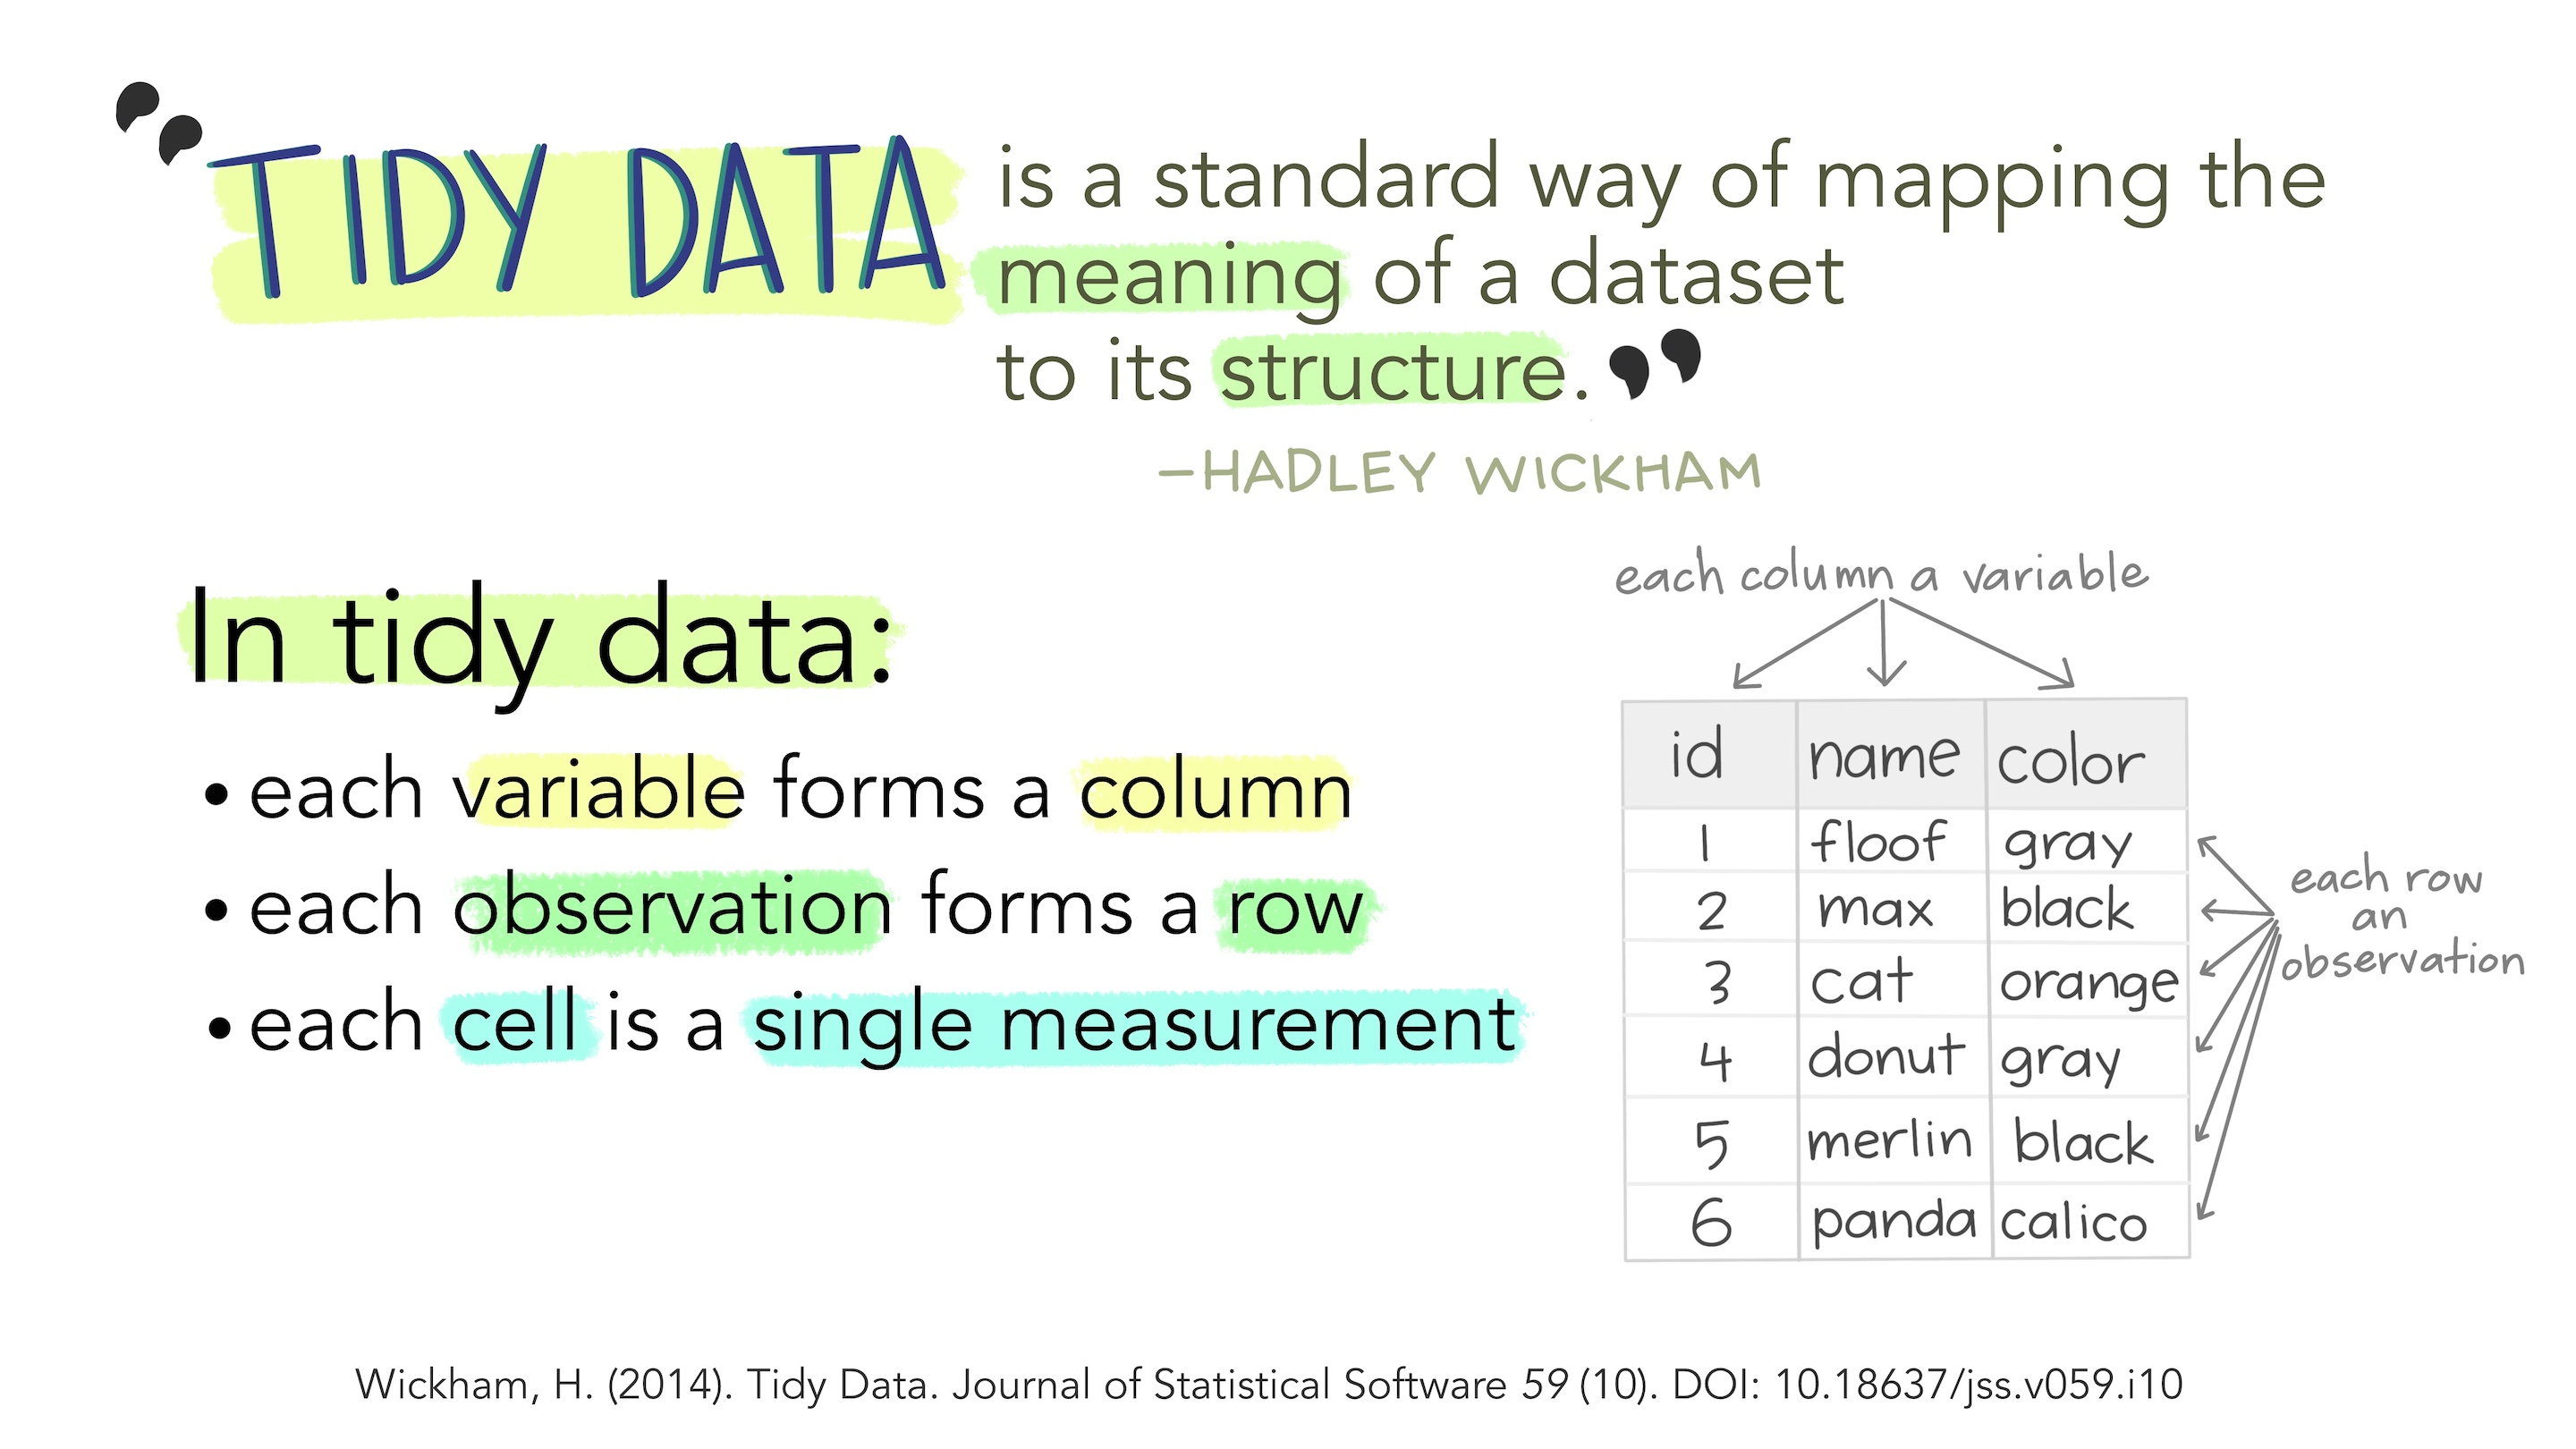
\includegraphics[width=6.25in,height=\textheight]{images/tidydata_1.jpg}

This may seem like a mundane topic, but tidy data provides a way of thinking about and organizing data that will become fundamental to how you input, wrangling, and work with environmental data - it becomes part of a systematic approach to working with data that \textbf{will make you a better data scientist and collaborator}.

\hypertarget{common-ways-data-are-untidy}{%
\section{Common ways data are untidy}\label{common-ways-data-are-untidy}}

One way to understand tidy data is to consider what makes some data sets \emph{untidy}. Let's explore some examples of untidy data, and for each think about (1) why it's untidy, and (2) how we would wrangle it to make it tidy data.

\hypertarget{untidy-example-1-a-single-variable-across-multiple-columns}{%
\subsection{Untidy example 1: A single variable across multiple columns}\label{untidy-example-1-a-single-variable-across-multiple-columns}}

One of the most common ways that data can be untidy is if a single variable is broken up by group across multiple columns. For example, the following data contains the weights of three dogs, measured over four years:

\begin{table}

\caption{\label{tab:unnamed-chunk-2}Dog weight (pounds) in untidy format, where a single variable (weight) is spread out across different levels of the year variable.}
\centering
\begin{tabular}[t]{l|r|r|r|r}
\hline
dog & 2018 & 2019 & 2020 & 2021\\
\hline
Teddy & 36.4 & 39.2 & 44.8 & 47.5\\
\hline
Khora & 41.6 & 48.3 & 52.9 & 50.1\\
\hline
Waffle & NA & NA & 20.4 & 23.7\\
\hline
\end{tabular}
\end{table}

In this example, there are really only 3 variables: dog name, dog weight, and year. But as organized, there are \textbf{5} columns - this should be our first indication that the data is not tidy. Instead of each variable occupying its own column, the \textbf{weight} measurements have been split up across multiple columns, separated by the different levels of \textbf{year}. Sometimes you will hear this called ``wide format'' when a single variable is spread across multiple columns.\\
~\\
\textbf{What would this data look like if it were tidy?}\\
~\\
To be in tidy data, each variable (\textbf{dog}, \textbf{weight}, and \textbf{year}) should have its own column. In this example, starting from the wide format data we need to reshape \textbf{weight} observations into a single column. Year will need to populate a new column, with year values repeated as necessary to align with the long-format weights. We'll also need to repeat the dog names to accommodate the number of observations for each.\\
~\\
Later on, we'll hear how to reshape data from wide-to-long format (e.g.~using \texttt{tidyr::pivot\_longer()} in R), but for now think about the tidy format of the same data, shown below:

\begin{table}

\caption{\label{tab:unnamed-chunk-3}Dog weight (pounds) in tidy format, where each variable is in its own column.}
\centering
\begin{tabular}[t]{l|l|r}
\hline
dog & year & weight\\
\hline
Teddy & 2018 & 36.4\\
\hline
Teddy & 2019 & 39.2\\
\hline
Teddy & 2020 & 44.8\\
\hline
Teddy & 2021 & 47.5\\
\hline
Khora & 2018 & 41.6\\
\hline
Khora & 2019 & 48.3\\
\hline
Khora & 2020 & 52.9\\
\hline
Khora & 2021 & 50.1\\
\hline
Waffle & 2018 & NA\\
\hline
Waffle & 2019 & NA\\
\hline
Waffle & 2020 & 20.4\\
\hline
Waffle & 2021 & 23.7\\
\hline
\end{tabular}
\end{table}

\hypertarget{untidy-example-2-multiple-values-in-a-single-cell}{%
\subsection{Untidy example 2: multiple values in a single cell}\label{untidy-example-2-multiple-values-in-a-single-cell}}

Another way that data can be untidy is if there are multiple ``measurements'' (or values) in a single cell. Keep in mind that a ``value'' doesn't have to be numeric - it's just a measurement or description for a recorded variable.

Sometimes raw data will contain multiple values in a single cell. For example, here we see that the make, model and year of cars are all in a single column called \textbf{type}:

\begin{table}

\caption{\label{tab:unnamed-chunk-4}Car descriptions in untidy format.}
\centering
\begin{tabular}[t]{l|l|l}
\hline
type & color & condition\\
\hline
1994 Toyota Corolla & silver & poor\\
\hline
2005 Subaru Outback & green & average\\
\hline
1977 Datsun 710 & blue & excellent\\
\hline
\end{tabular}
\end{table}

An important thing is to be future-thinking about data, and expect that \textbf{even if you don't think a specific question is important now, it may be important in the future} -- and having data in tidy format will make it easier to answer a wider range of questions with limited frustration. For example, maybe in the future (and if this were part of a larger data set) we would want to assess the condition of cars by year, or the color of cars by make and model. No matter how you slice those questions, having each variable in its own column will make them easier to explore and answer with code.\\
~\\
In the future, you'll learn how to separate components of a single column into multiple columns (e.g.~using the \texttt{tidyr::separate()} function), which in this example would help to create a tidy version of the data that looks like this:\\

\begin{table}

\caption{\label{tab:unnamed-chunk-5}Car descriptions in tidy format.}
\centering
\begin{tabular}[t]{l|l|l|l|l}
\hline
year & make & model & color & condition\\
\hline
1994 & Toyota & Corolla & silver & poor\\
\hline
2005 & Subaru & Outback & green & average\\
\hline
1977 & Datsun & 710 & blue & excellent\\
\hline
\end{tabular}
\end{table}

\textbf{Untidy example 3: multiple observations in a single row}

Occasionally, you will see environmental data where information for \emph{multiple observations are stored in a single row}. For example, this is common when research divers are estimating numbers of a certain species within different size bins. For example, a dive record may contain information like this:

\begin{table}

\caption{\label{tab:unnamed-chunk-6}Spiny lobster counts by size.}
\centering
\begin{tabular}[t]{l|r|r}
\hline
species & size\_cm & count\\
\hline
spiny lobster & 4.5 & 2\\
\hline
spiny lobster & 5.0 & 4\\
\hline
spiny lobster & 5.5 & 0\\
\hline
spiny lobster & 6.0 & 1\\
\hline
spiny lobster & 6.5 & 3\\
\hline
\end{tabular}
\end{table}

So in this case, we have multiple lobster observations occupying single rows (e.g.~the second row actually contains data for four lobsters). On the spectrum of untidy data, this isn't too bad - but it can make it much easier (and less risky) to visualize and analyze the data if each observation is in its own row. We'll learn how to convert a \textbf{frequency table} (like this one, which contains counts) into \textbf{case format} (which does have a single row per observation, so that the data look something like this:

\begin{table}[H]
\centering
\begin{tabular}{l|r}
\hline
species & size\_cm\\
\hline
spiny lobster & 4.5\\
\hline
spiny lobster & 4.5\\
\hline
spiny lobster & 5.0\\
\hline
spiny lobster & 5.0\\
\hline
spiny lobster & 5.0\\
\hline
spiny lobster & 5.0\\
\hline
spiny lobster & 6.0\\
\hline
spiny lobster & 6.5\\
\hline
spiny lobster & 6.5\\
\hline
spiny lobster & 6.5\\
\hline
\end{tabular}
\end{table}

Now, each individual lobster occupies its own row, and the data are in tidy format.

\hypertarget{tidy-data-makes-coding-easier}{%
\section{Tidy data makes coding easier}\label{tidy-data-makes-coding-easier}}

The process of creating tidy data is useful in an of itself, because it requires us to be deliberate and thoughtful about how we structure our data, and makes us define our \emph{variables}, \emph{observations} and \emph{measurements}. We will learn why that benefits us and our collaborators in the next section. Here, let's learn why tidy data is code- and coder-friendly.

\hypertarget{code-working-for-you}{%
\subsection{Code working for you}\label{code-working-for-you}}

\hypertarget{parse-explore}{%
\subsection{Parse \& explore}\label{parse-explore}}

\hypertarget{safer-summary-statistics}{%
\subsection{Safer summary statistics}\label{safer-summary-statistics}}

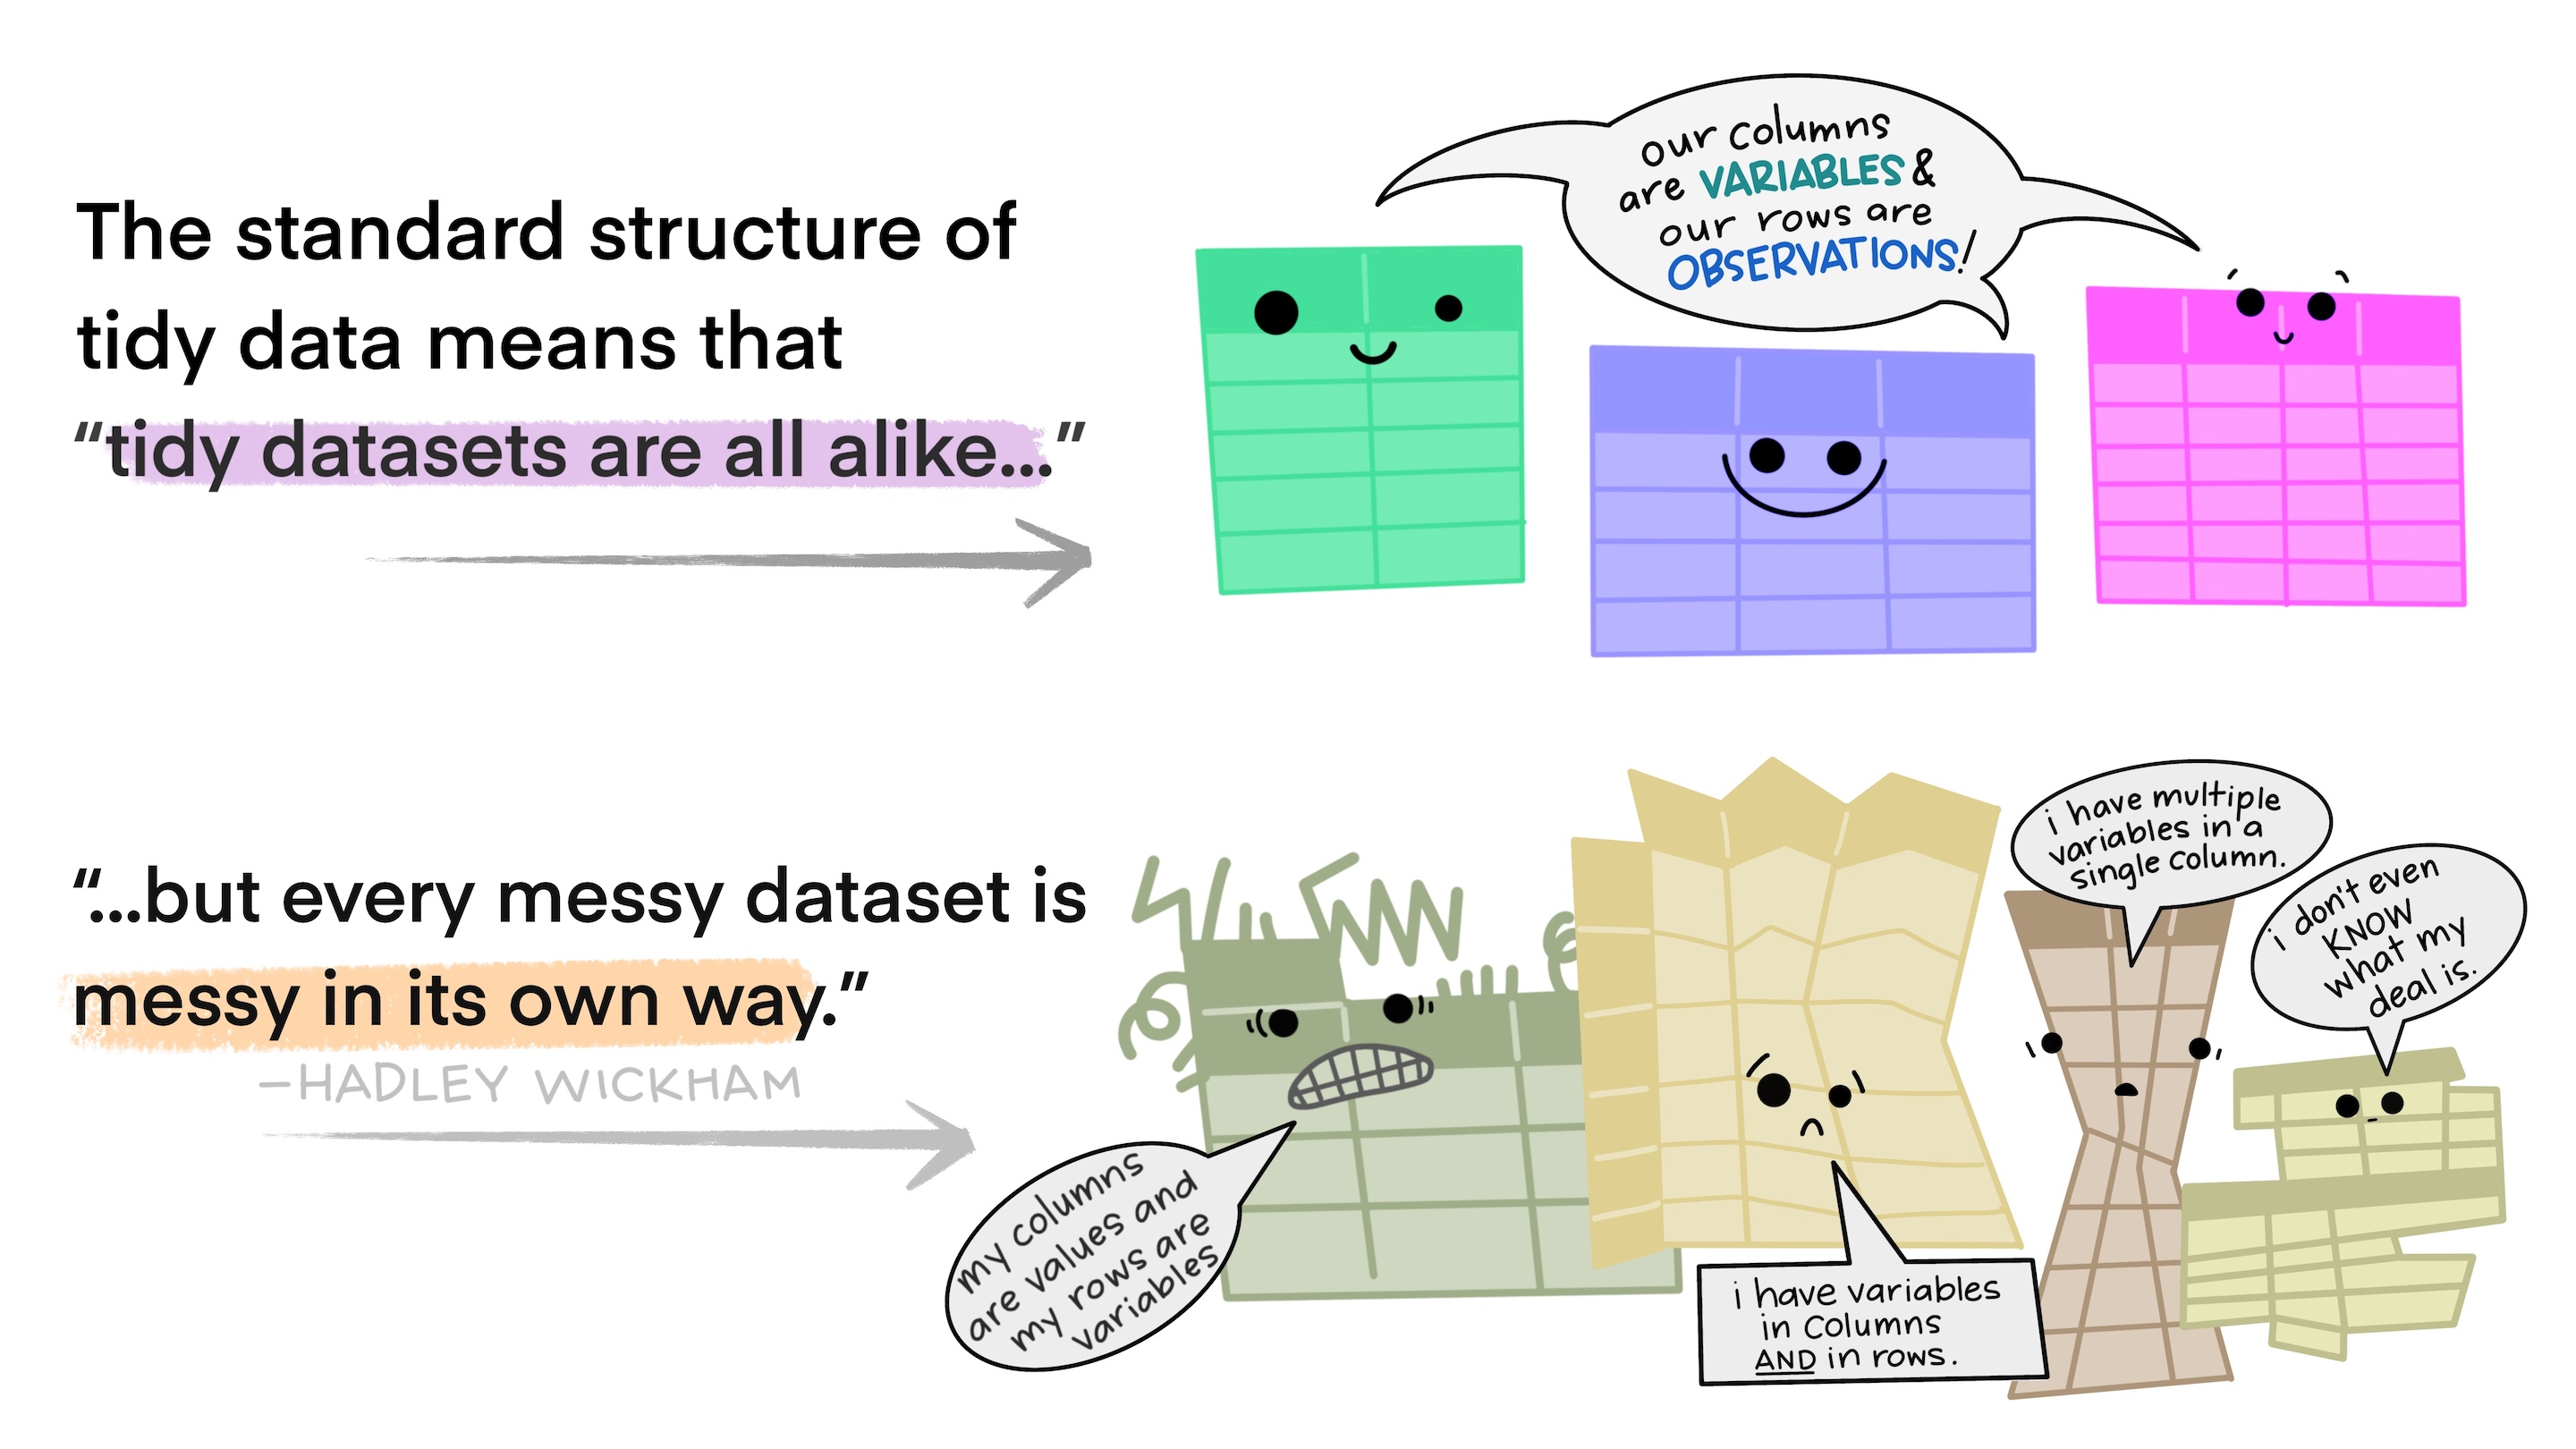
\includegraphics[width=6.26042in,height=\textheight]{images/tidydata_2.jpg}

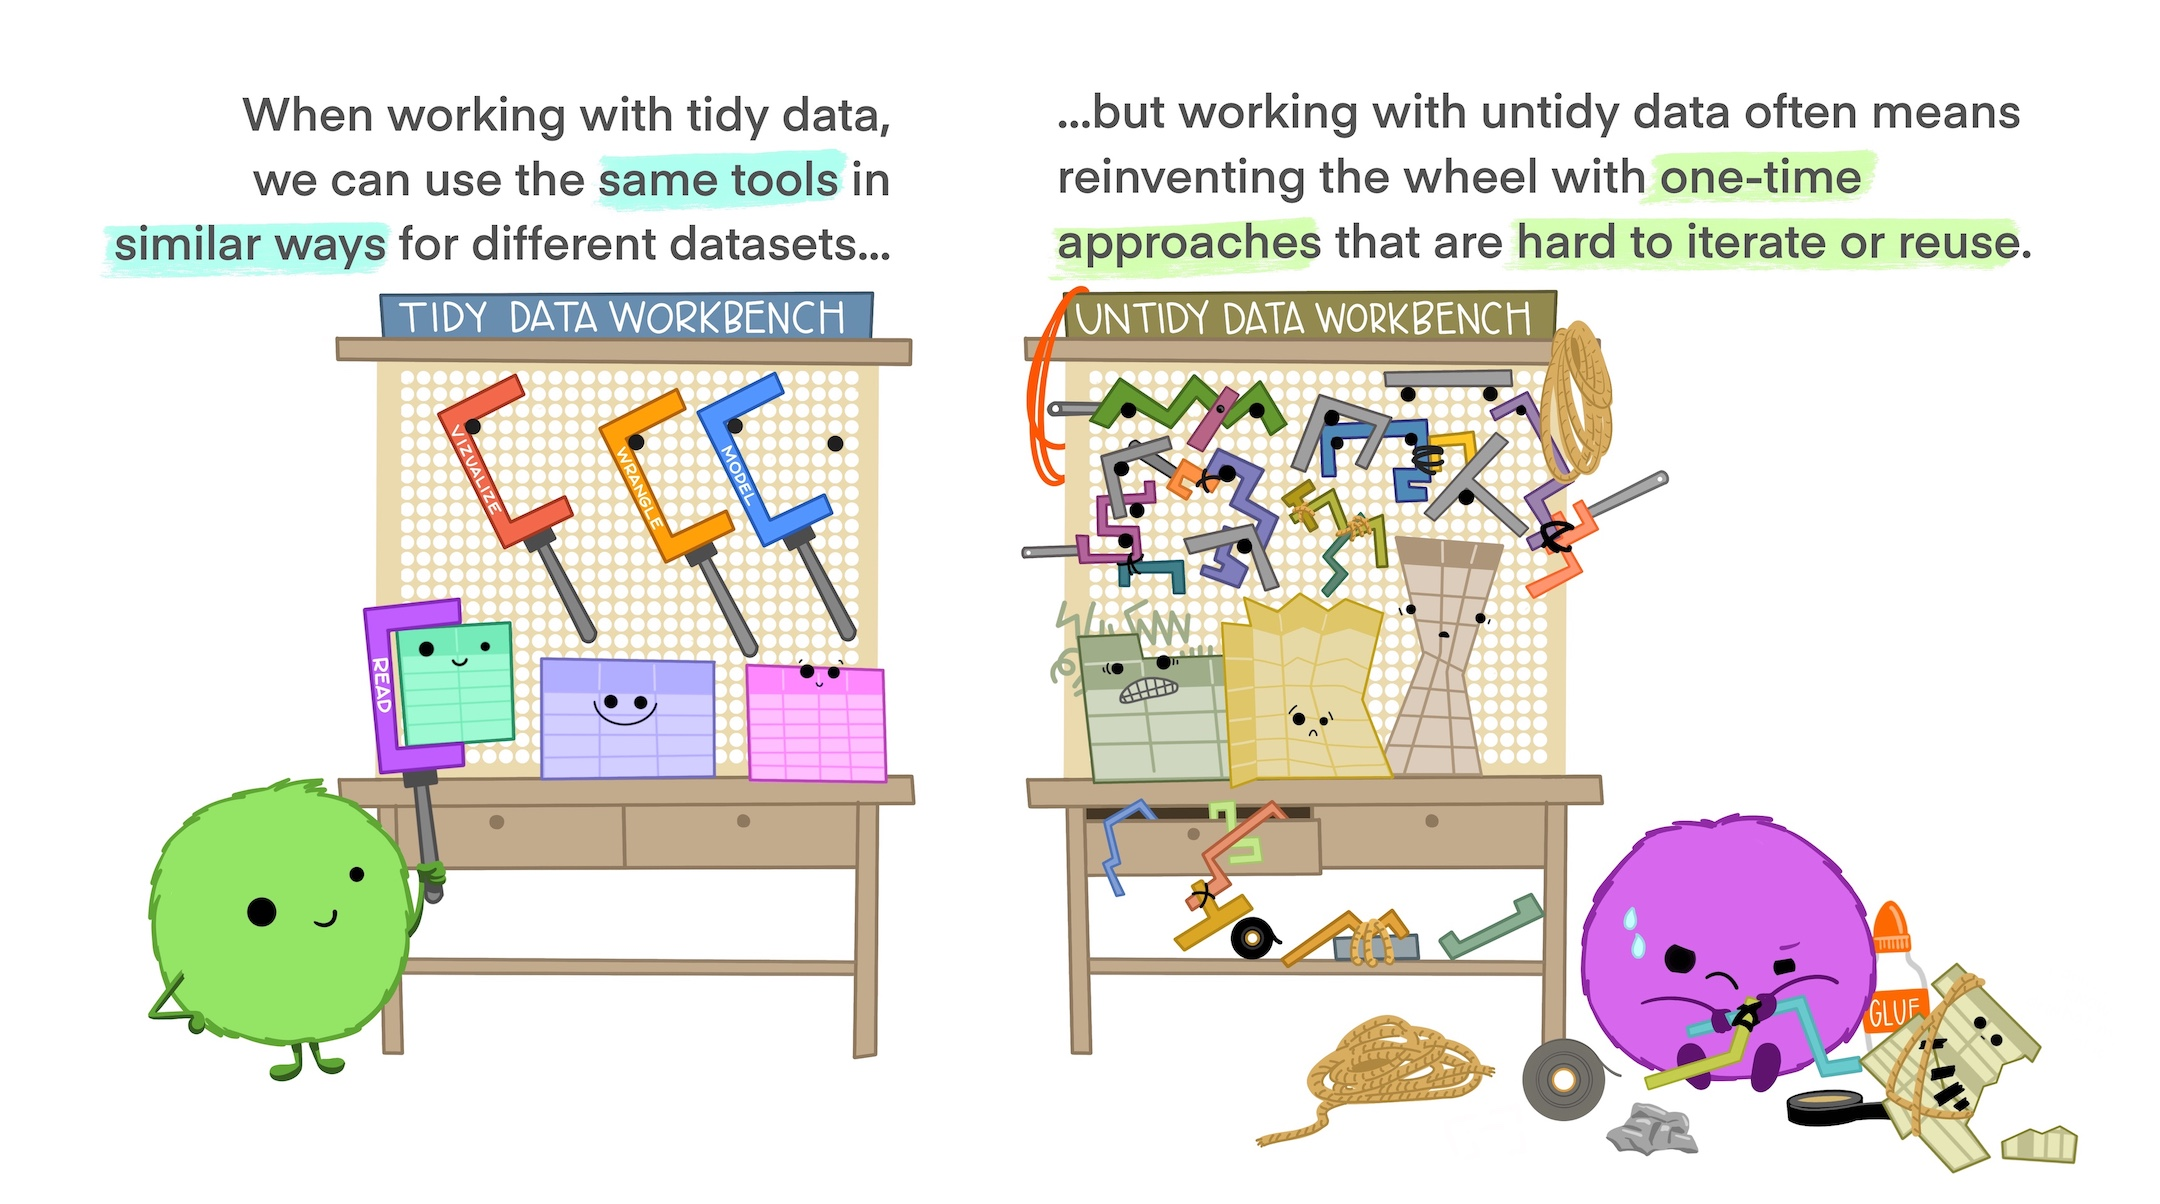
\includegraphics{images/tidydata_3.jpg}

\hypertarget{tidy-data-for-collaboration}{%
\section{Tidy data for collaboration}\label{tidy-data-for-collaboration}}

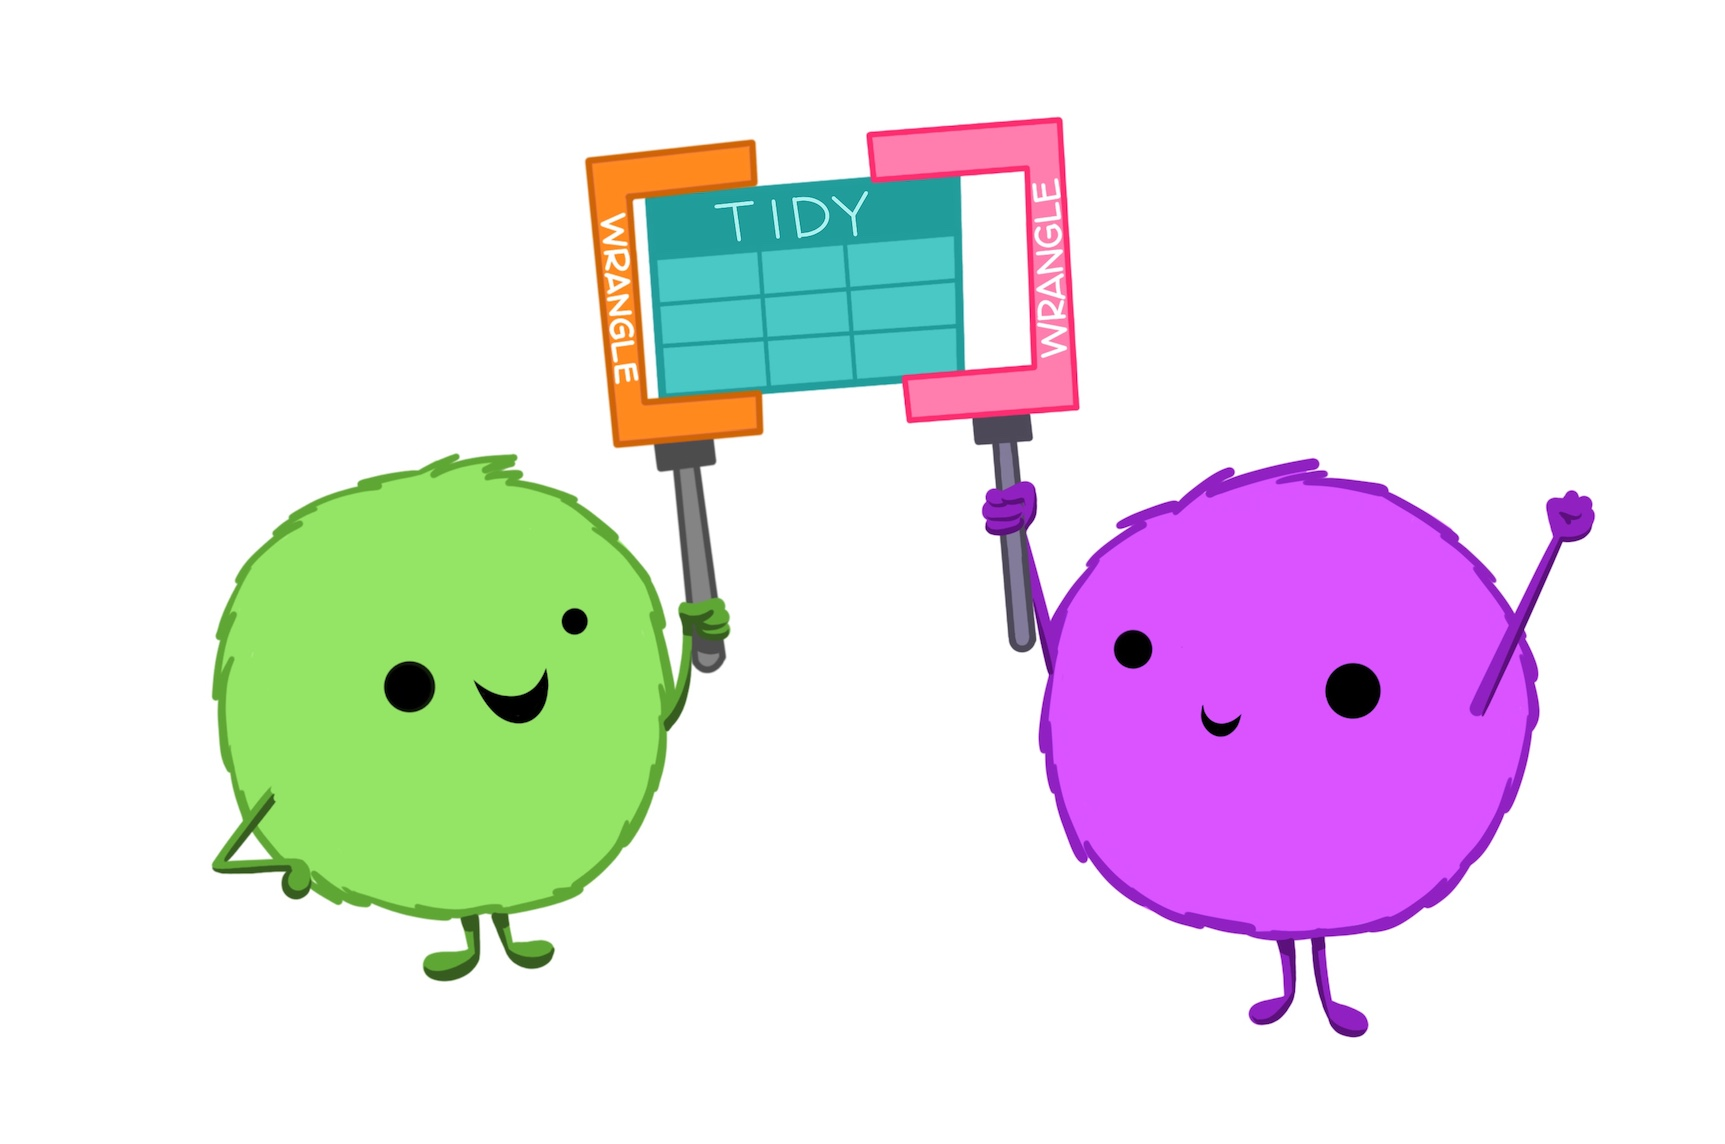
\includegraphics[width=5.22917in,height=\textheight]{images/tidydata_4.jpg}

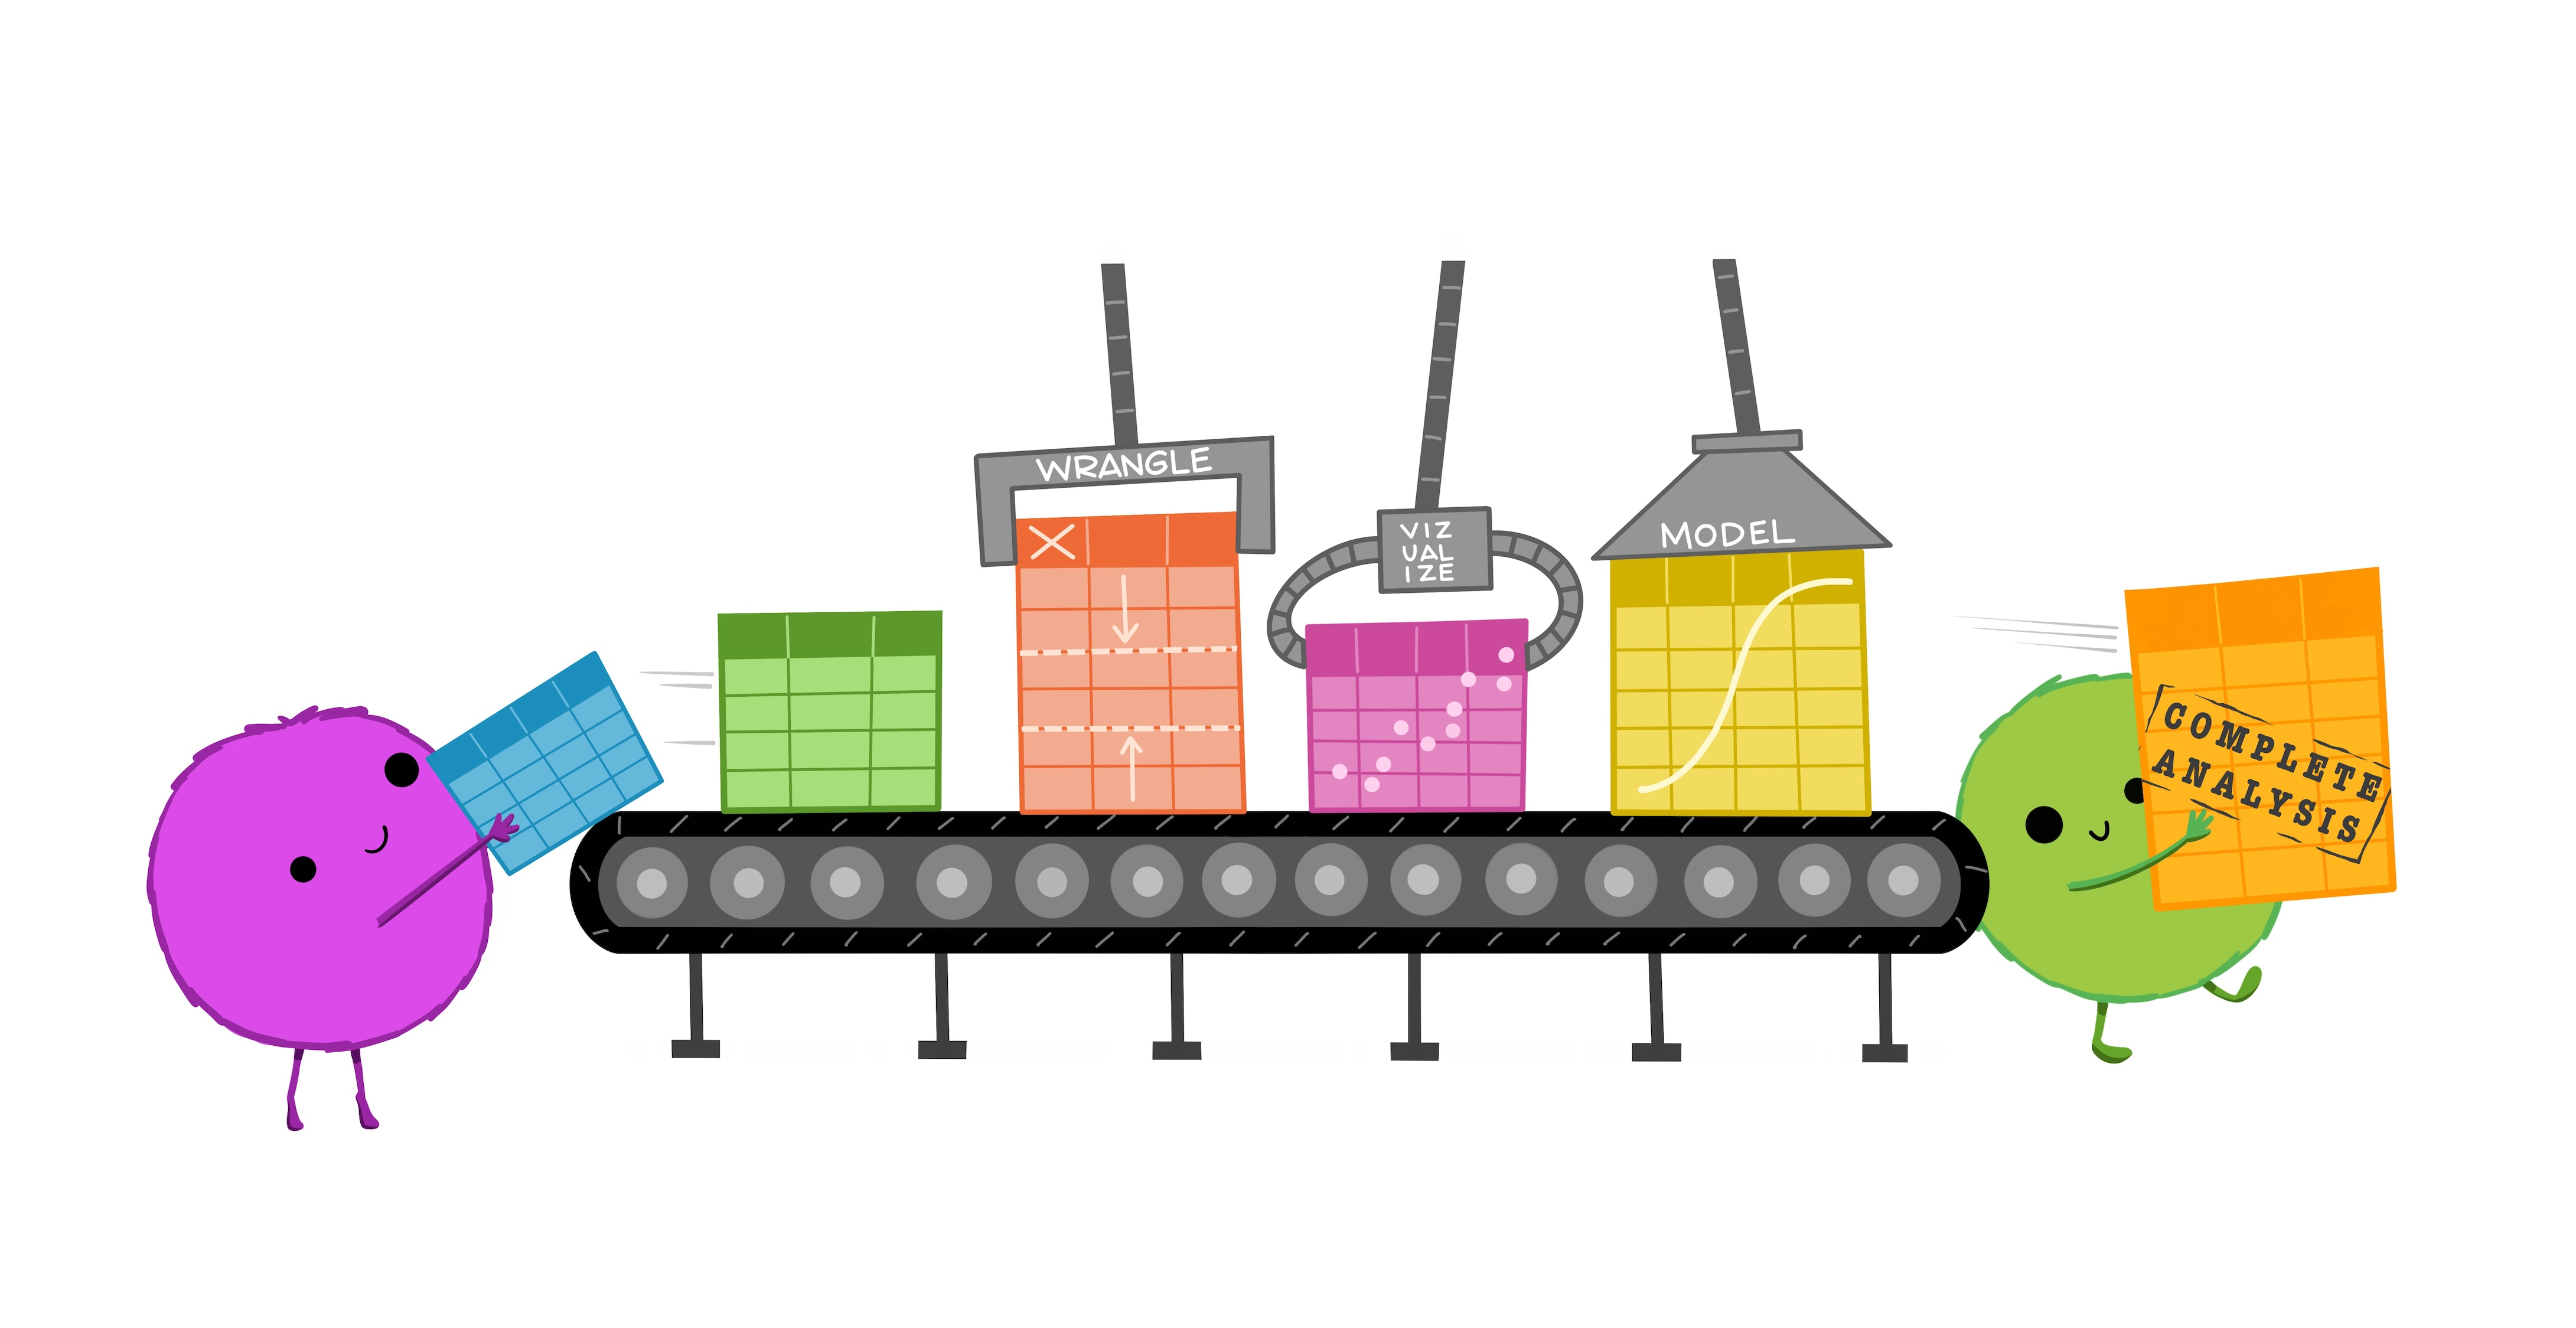
\includegraphics{images/tidydata_5.jpg}

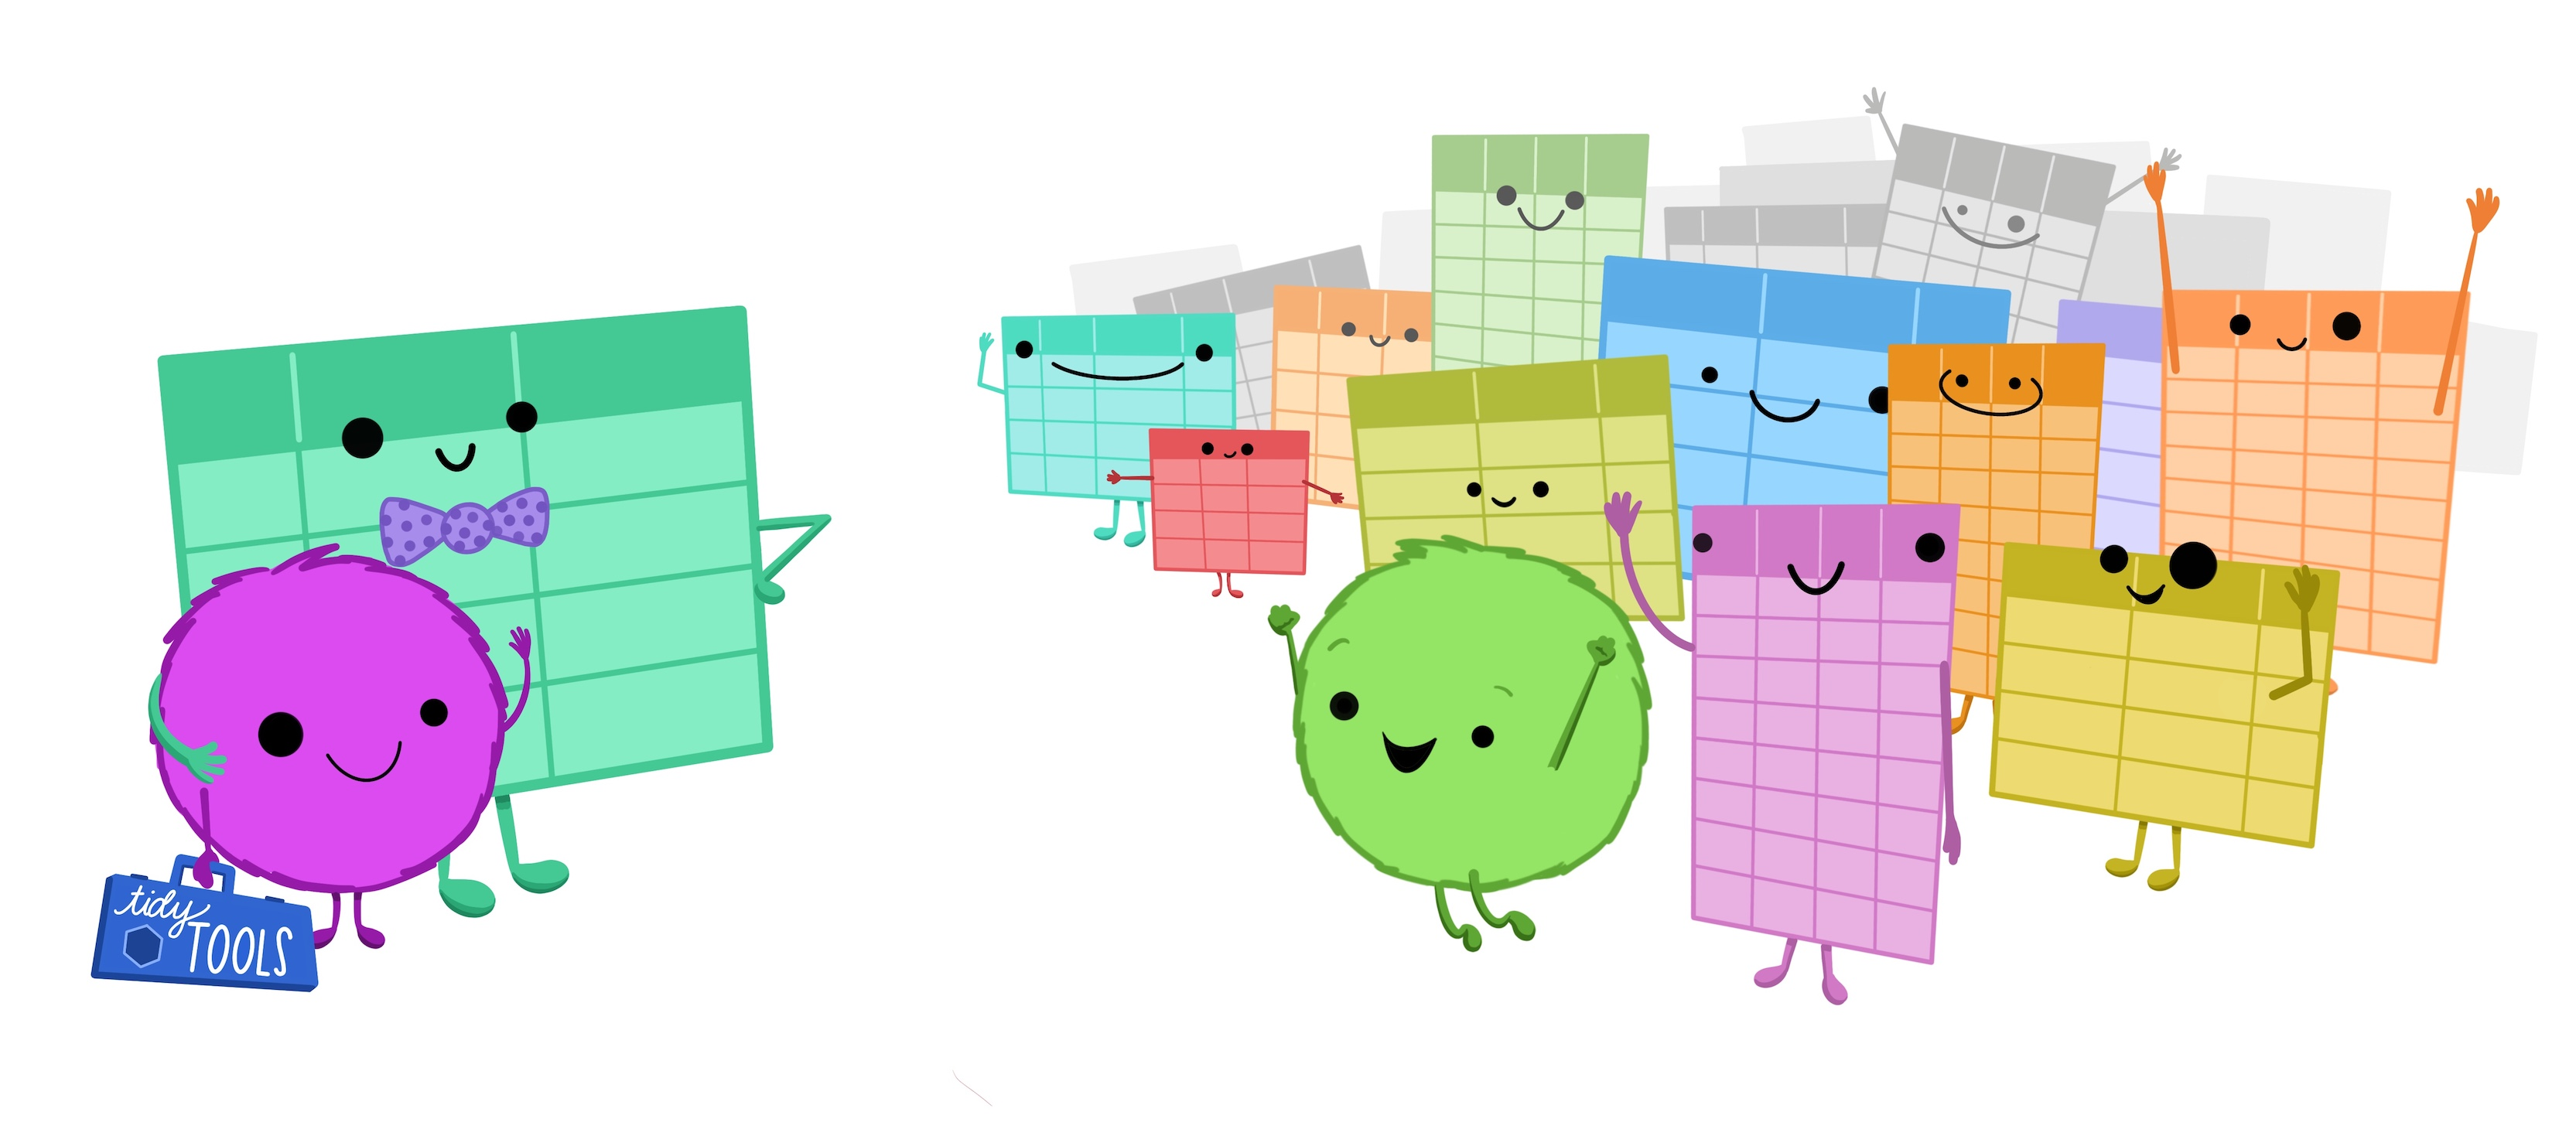
\includegraphics{images/tidydata_6.jpg}

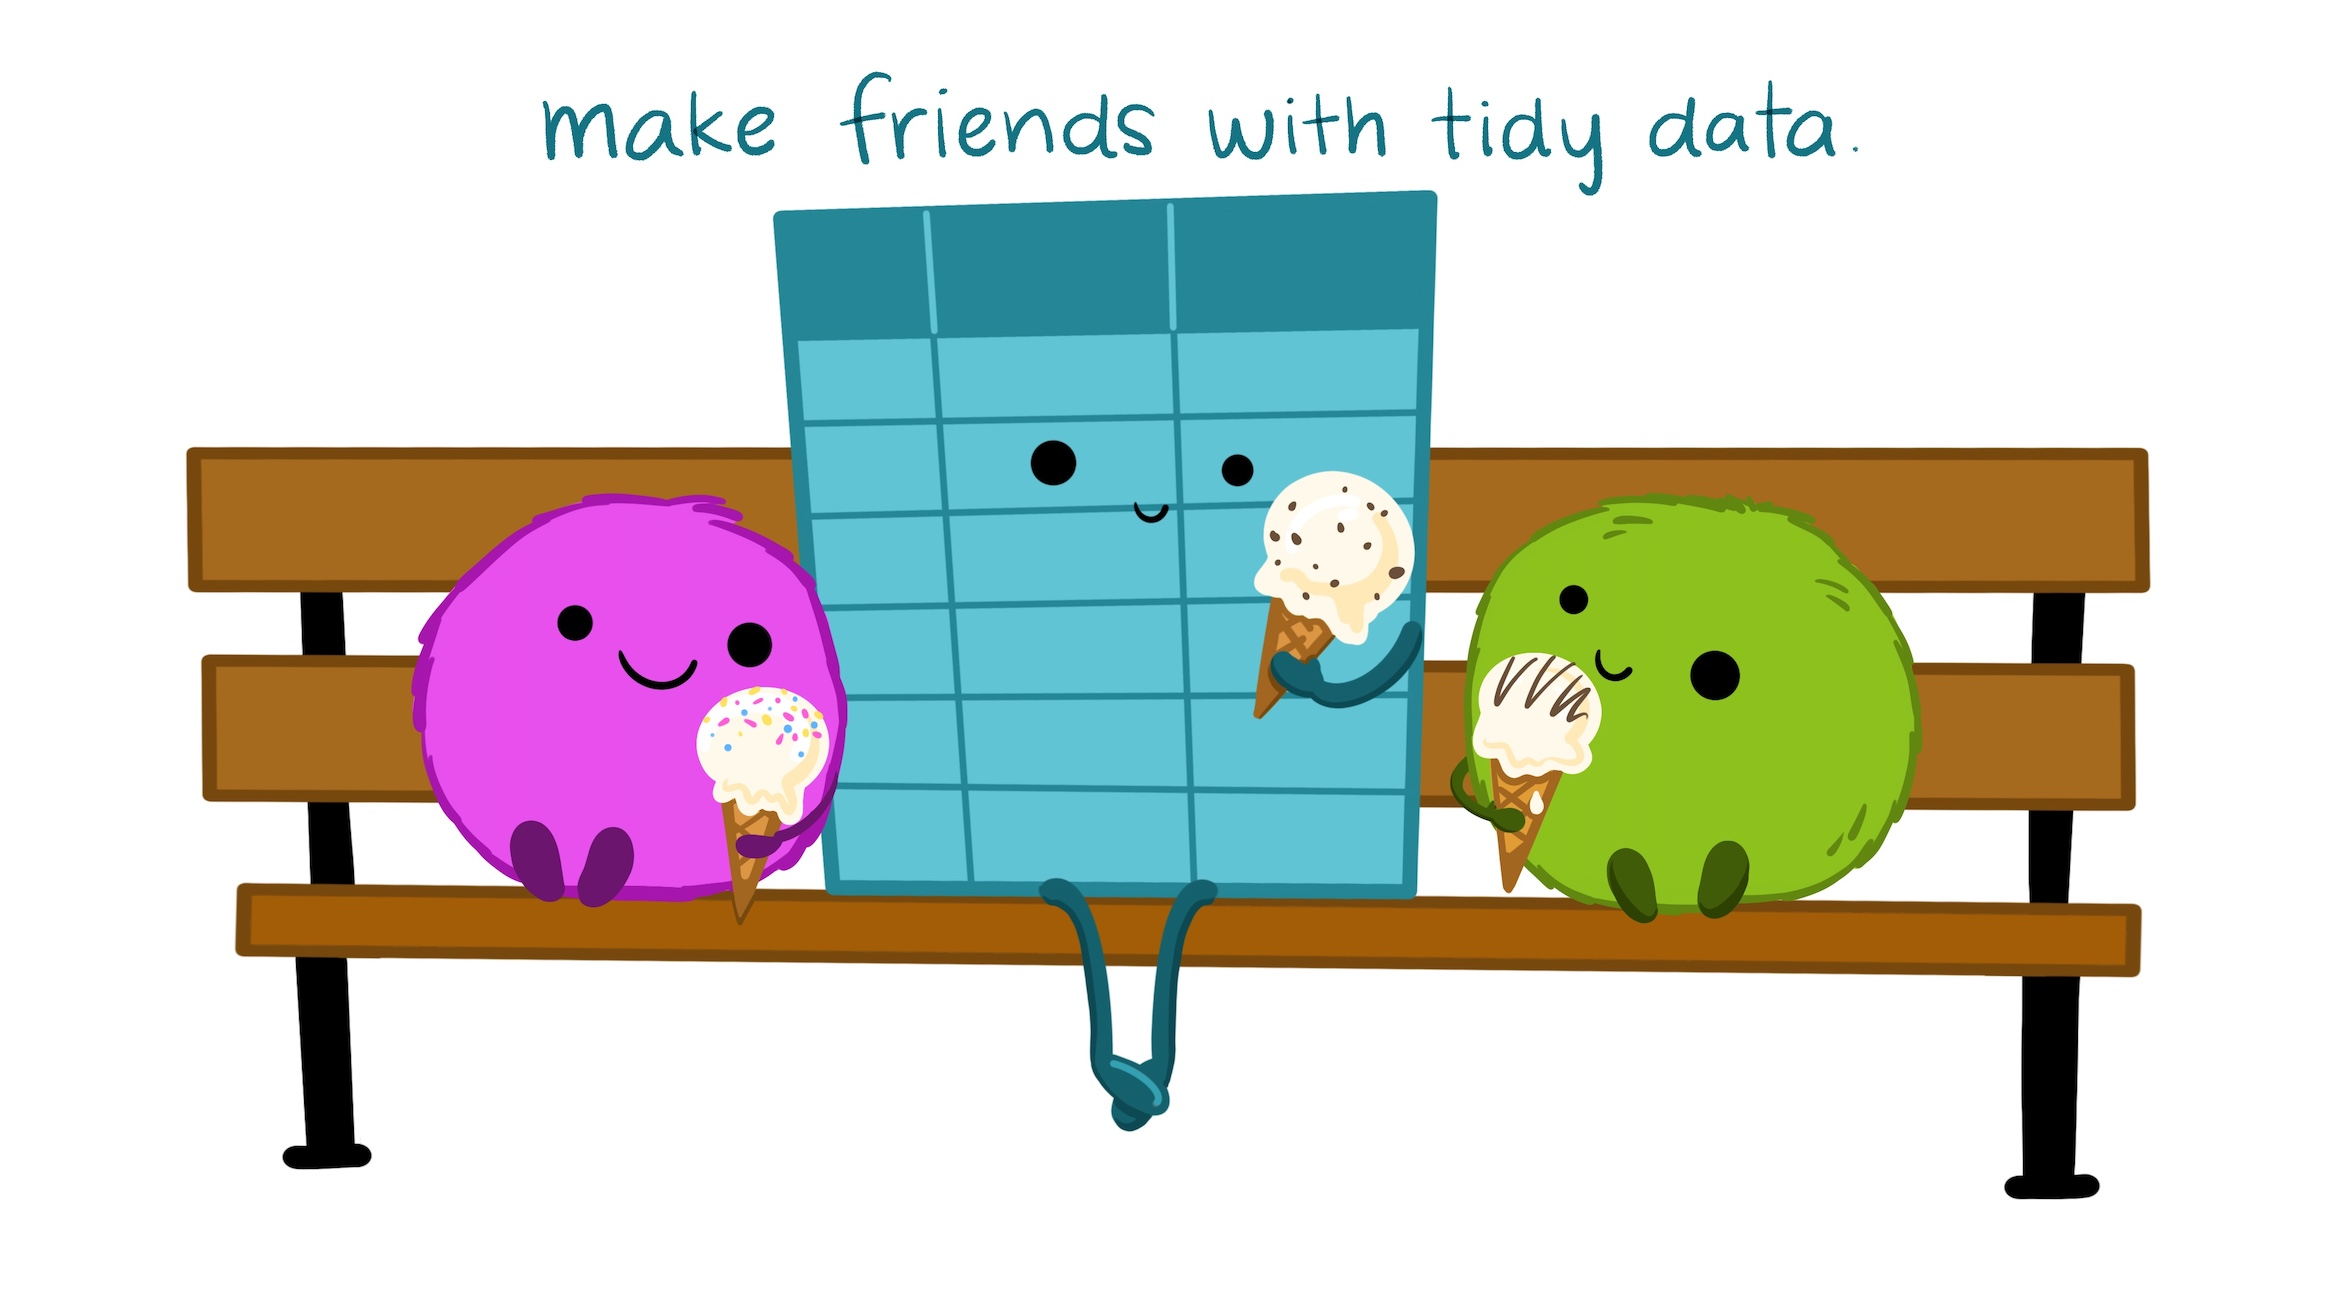
\includegraphics{images/tidydata_7.jpg}

\hypertarget{basic-wrangling}{%
\chapter{Basic wrangling}\label{basic-wrangling}}

Indexing, subsetting, etc.

\hypertarget{logicals}{%
\chapter{Logical operators}\label{logicals}}

\hypertarget{conditionals}{%
\chapter{Conditionals}\label{conditionals}}

\hypertarget{iteration}{%
\chapter{Iteration}\label{iteration}}

From Miriam-Webster Dictionary:

"\textbf{Iteration:} (\emph{noun}) the action or a process of iterating or repeating, such as:

\begin{itemize}
\tightlist
\item
  a procedure in which repetition of a sequence of operations yields results successively closer to a desired result
\item
  the repetition of a sequence of computer instructions a specified number of times or until a condition is met"
\end{itemize}

\hypertarget{iteration-in-programming}{%
\section{Iteration in programming}\label{iteration-in-programming}}

In programming, iteration is repeating instructions. Usually it's to spare yourself from having to manually do a repetitious thing. Well-written iteration can also make code more readable, usable, and efficient (definitely to write, sometimes to run).

For example, let's consider a few scenarios that may prompt you to use iteration:

\begin{itemize}
\tightlist
\item
  Your data contains 382 columns (variables), and you want to find the mean and standard deviation for each variable
\item
  You have 250 csv files and you want to read them all in and combine them into a single data frame
\item
  In a single data frame you have annual observations for fish passage from 1970 - 2019 recorded at 25 dams in Oregon, and you want to create and save a single graph for passage at each dam
\end{itemize}

\ldots so basically, anything where you're like ``Welp, I guess I'm going to be doing the same thing over and over and over and over\ldots{}'' should inspire you to consider iteration.

\hypertarget{a-real-world-example-of-iteration-in-environmental-data-science}{%
\subsection{A real-world example of iteration in environmental data science}\label{a-real-world-example-of-iteration-in-environmental-data-science}}

\hypertarget{generic-for-loop-anatomy}{%
\section{Generic for loop anatomy}\label{generic-for-loop-anatomy}}

When we iterate in code, most often that means we're writing some version of a for loop, which we can read as ``For these elements in this thing, do this thing to each and return the output, then move on to the next element until you reach the end or a stopping point.'' There are a bunch of variations on that, but that's the overarching idea.

For example, in the image below our vector is a parade of friendly monsters getting passed through a for loop. There are conditions within the for loop dictating which type of accessory each monster will get, based on their shape. Then the outcome is returned with \texttt{print()}.

\begin{figure}
\centering
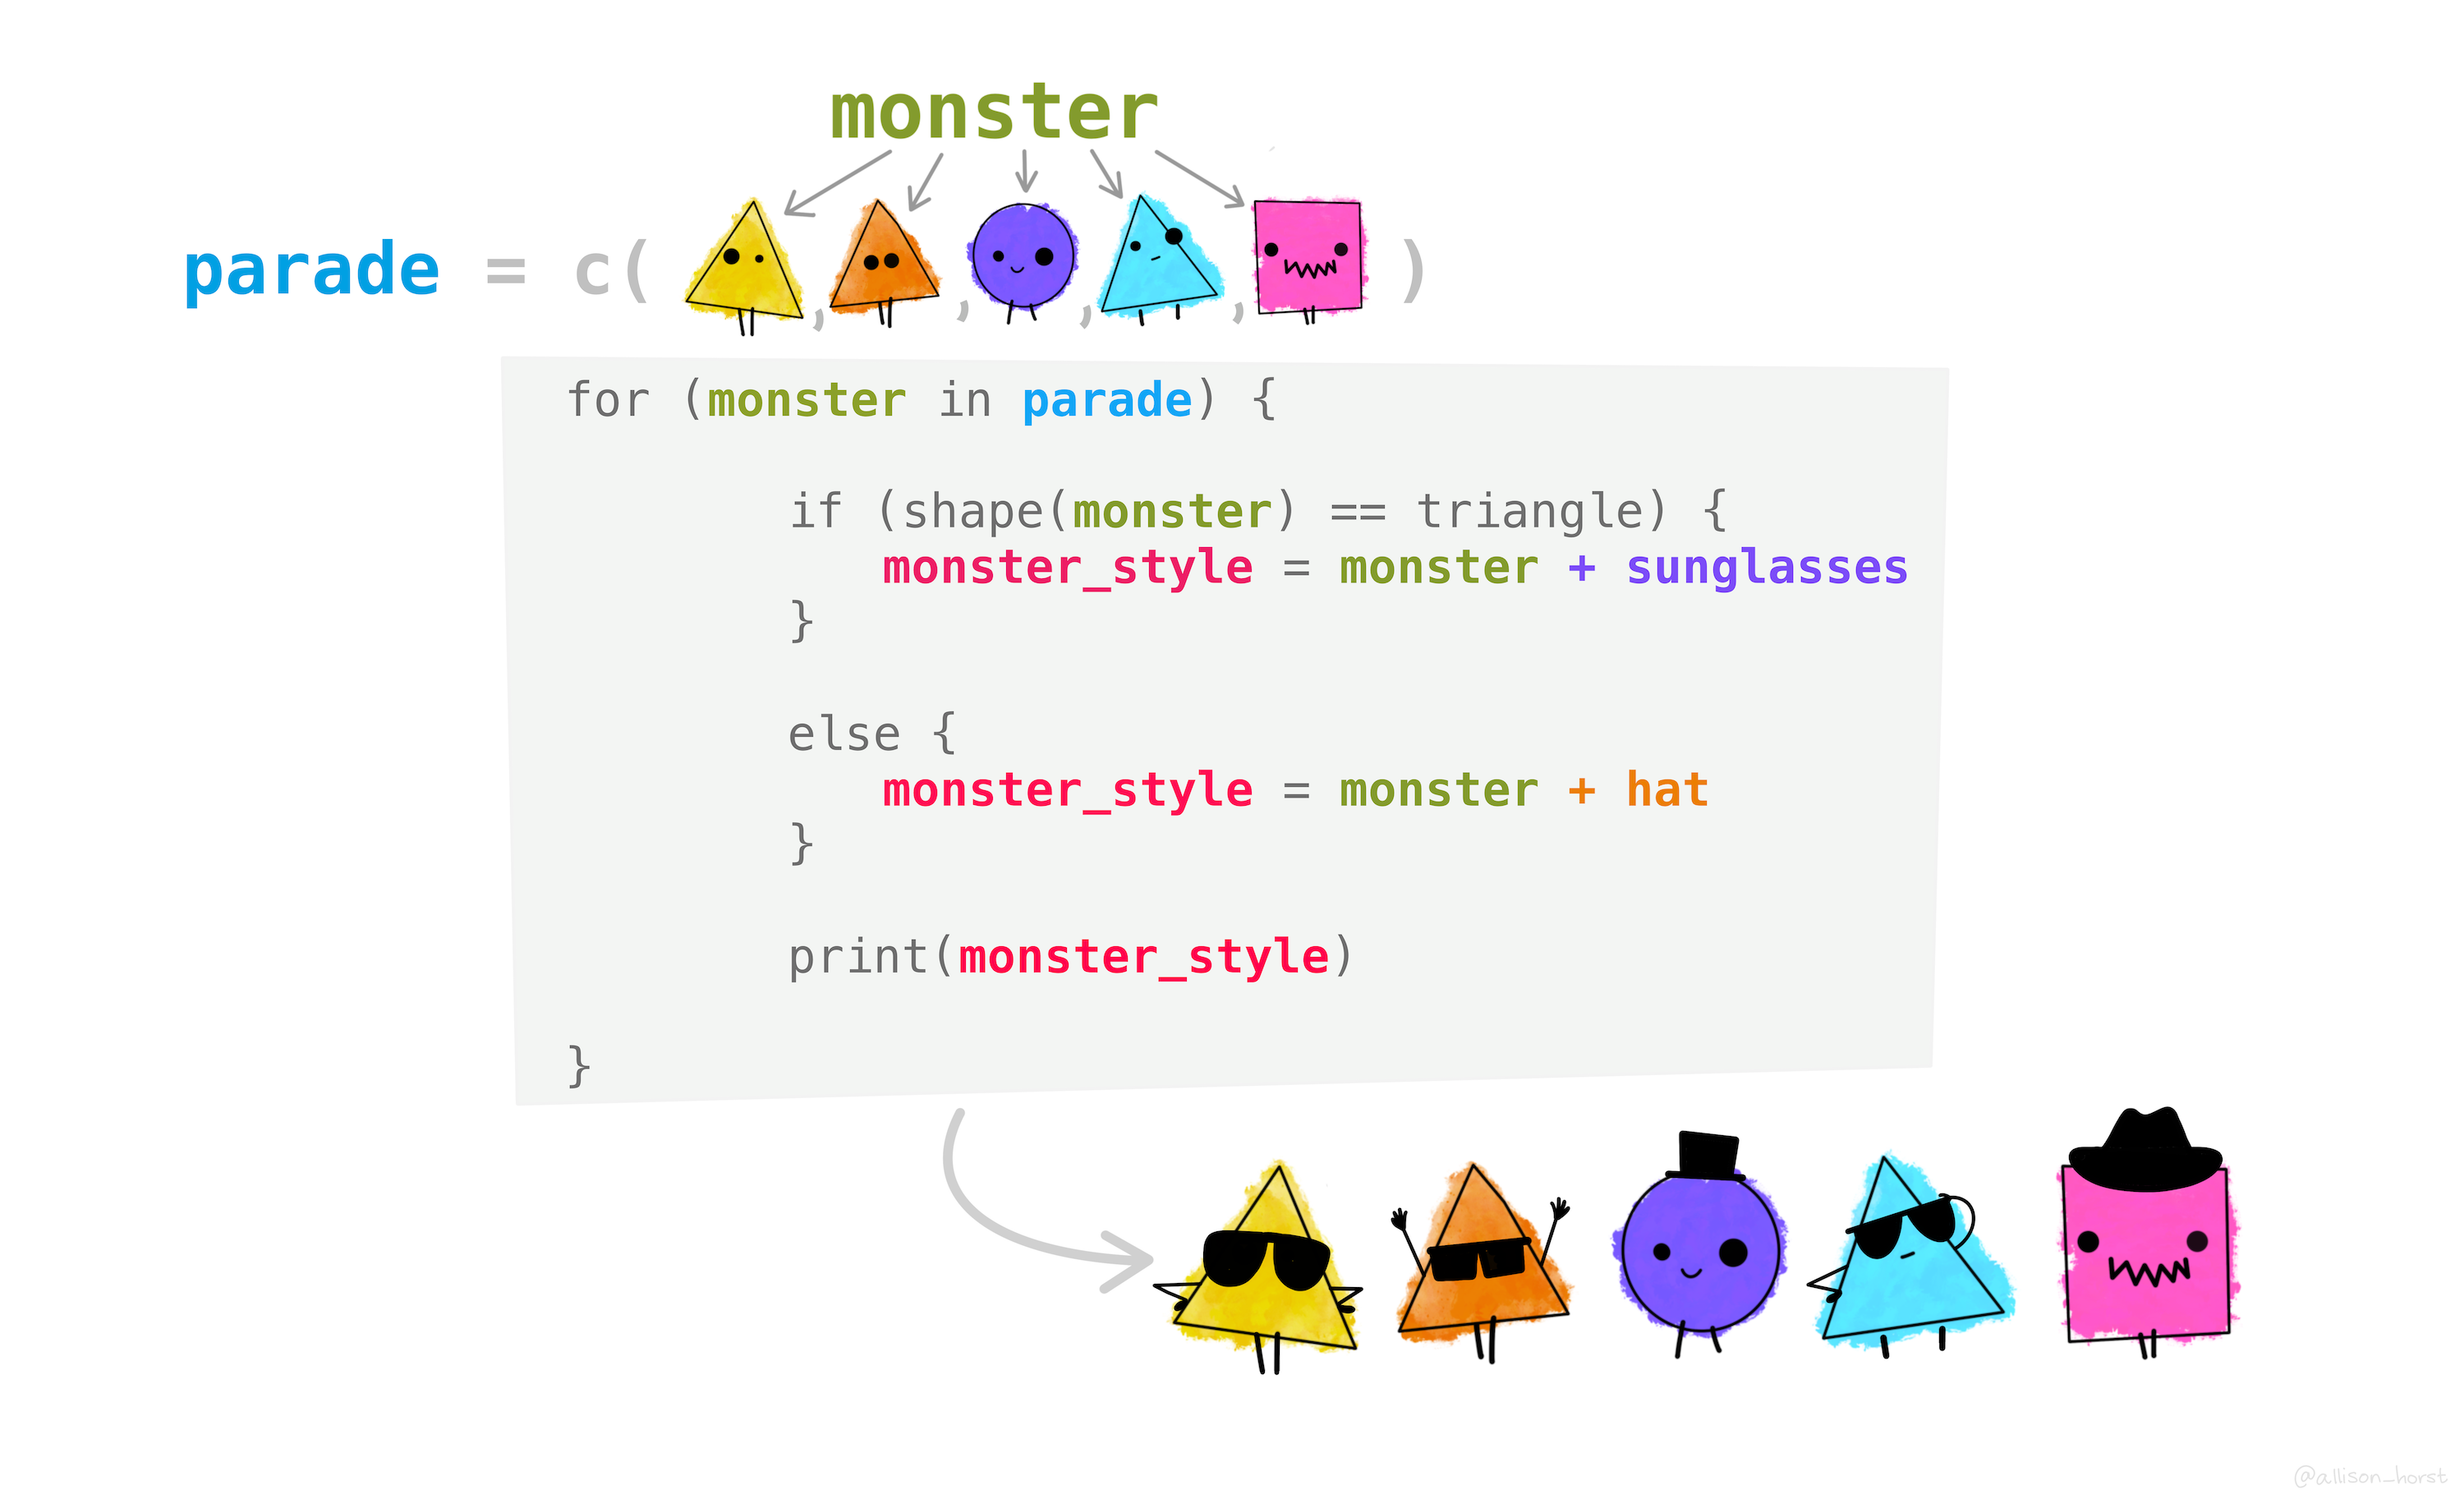
\includegraphics[width=6.96875in,height=\textheight]{images/for_loop_monsters.png}
\caption{Monsters passing through a for loop, getting assigned sunglasses or a hat based on their shape.}
\end{figure}

In words, how can we describe what's happening in this for loop? As each monster is passed individually through the loop, \textbf{if it is a triangle}, then it gets sunglasses added to it -- that's why the first element in the output vector is a triangle monster with sunglasses. Then we move on to the second (orange) monster. Since they are also a triangle, they're assigned sunglasses. However, when we get to the \textbf{third} (purple) monster, it is \textbf{not} a triangle, and anything monster shape other than a triangle is assigned a \textbf{hat} - so we see the third output is the purple circle monster with a hat.

\ldots and so on until all elements have been passed through the for loop or a stopping point is otherwise reached.

\hypertarget{anatomy-of-a-for-loop}{%
\subsection{Anatomy of a for loop}\label{anatomy-of-a-for-loop}}

\hypertarget{basic-for-loops-in-r-and-python}{%
\section{Basic for loops in R and Python}\label{basic-for-loops-in-r-and-python}}

Let's take a look at some basic for loops, written in both R and Python.

\hypertarget{example-a-vector-of-very-good-dogs}{%
\subsubsection{Example: A vector of very good dogs}\label{example-a-vector-of-very-good-dogs}}

Here's our scenario: starting with a vector of dog names ``Teddy'', ``Khora'', and ``Waffle'', write a for loop that returns the statement ``{[}dog name here{]} is a very good dog!''

\textbf{In R:}

\begin{Shaded}
\begin{Highlighting}[]
\CommentTok{\# Create the vector of names:}
\NormalTok{dog\_names }\OtherTok{\textless{}{-}} \FunctionTok{c}\NormalTok{(}\StringTok{"Teddy"}\NormalTok{, }\StringTok{"Khora"}\NormalTok{, }\StringTok{"Waffle"}\NormalTok{)}

\CommentTok{\# Run it through the loop:}
\ControlFlowTok{for}\NormalTok{ (i }\ControlFlowTok{in}\NormalTok{ dog\_names) \{}
  \FunctionTok{print}\NormalTok{(}\FunctionTok{paste}\NormalTok{(i, }\StringTok{"is a very good dog!"}\NormalTok{))}
\NormalTok{\}}
\end{Highlighting}
\end{Shaded}

\begin{verbatim}
## [1] "Teddy is a very good dog!"
## [1] "Khora is a very good dog!"
## [1] "Waffle is a very good dog!"
\end{verbatim}

\textbf{In Python:}

\begin{Shaded}
\begin{Highlighting}[]
\CommentTok{\# Create the vector of names:}
\NormalTok{dog\_names }\OperatorTok{=}\NormalTok{ [}\StringTok{\textquotesingle{}Teddy\textquotesingle{}}\NormalTok{, }\StringTok{\textquotesingle{}Khora\textquotesingle{}}\NormalTok{, }\StringTok{\textquotesingle{}Waffle\textquotesingle{}}\NormalTok{]}

\CommentTok{\# Run it through the for loop:}
\ControlFlowTok{for}\NormalTok{ i }\KeywordTok{in}\NormalTok{ dog\_names:}
    \BuiltInTok{print}\NormalTok{(i }\OperatorTok{+} \StringTok{" is a very good dog!"}\NormalTok{)}
\end{Highlighting}
\end{Shaded}

\begin{verbatim}
## Teddy is a very good dog!
## Khora is a very good dog!
## Waffle is a very good dog!
\end{verbatim}

Note that there's nothing special about \texttt{i} here - that's just an identifier for ``each element in this vector''. It can be whatever object name you want, but make sure you're referring to the correct thing later on in the loop body. For example, that code could have been written in R as:

\begin{Shaded}
\begin{Highlighting}[]
\ControlFlowTok{for}\NormalTok{ (treats }\ControlFlowTok{in}\NormalTok{ dog\_names) \{}
  \FunctionTok{print}\NormalTok{(}\FunctionTok{paste}\NormalTok{(treats, }\StringTok{"is a very good dog!"}\NormalTok{))}
\NormalTok{\}}
\end{Highlighting}
\end{Shaded}

\hypertarget{example-hypotenuses}{%
\subsubsection{Example: Hypotenuses!}\label{example-hypotenuses}}

For a vector of values \texttt{2,\ 3,\ 4,\ 5,\ 6,\ 7}, for any two sequential values, find the length of the hypotenuse if the two values are the lengths of sides of a right triangle. In other words, we'll find the hypotenuse length for right triangles with side lengths 2 \& 3, 3 \& 4, 4 \& 5, etc.

Recall the Pythagorean theorem:

\[a^2 + b^2 = c^2\]

\textbf{In R:}

\begin{Shaded}
\begin{Highlighting}[]
\CommentTok{\# Make the vector of values: }
\NormalTok{triangle\_sides }\OtherTok{\textless{}{-}} \FunctionTok{c}\NormalTok{(}\DecValTok{2}\NormalTok{, }\DecValTok{3}\NormalTok{, }\DecValTok{4}\NormalTok{, }\DecValTok{5}\NormalTok{, }\DecValTok{6}\NormalTok{, }\DecValTok{7}\NormalTok{)}

\CommentTok{\# Create the loop to calculate the hypotenuses: }
\ControlFlowTok{for}\NormalTok{ (i }\ControlFlowTok{in} \DecValTok{1}\SpecialCharTok{:}\NormalTok{(}\FunctionTok{length}\NormalTok{(triangle\_sides) }\SpecialCharTok{{-}} \DecValTok{1}\NormalTok{)) \{}
\NormalTok{  hypotenuse }\OtherTok{=} \FunctionTok{sqrt}\NormalTok{(triangle\_sides[i]}\SpecialCharTok{\^{}}\DecValTok{2} \SpecialCharTok{+}\NormalTok{ triangle\_sides[i }\SpecialCharTok{+} \DecValTok{1}\NormalTok{]}\SpecialCharTok{\^{}}\DecValTok{2}\NormalTok{)}
  \FunctionTok{print}\NormalTok{(hypotenuse)}
\NormalTok{\}}
\end{Highlighting}
\end{Shaded}

\begin{verbatim}
## [1] 3.605551
## [1] 5
## [1] 6.403124
## [1] 7.81025
## [1] 9.219544
\end{verbatim}

\textbf{In Python:}

Recall: Python indexing starts at ZERO (i.e., the first element in a vector is referenced with \texttt{vec{[}0{]}}), and the syntax for raising something to a power is \texttt{**} (e.g.~\texttt{x**2}).

\textbf{A weird one:} the \texttt{range()} function in Python ``\ldots returns a sequence of numbers, starting from 0 by default, and increments by 1 (by default), and stops \textbf{before} a specified number.'' So to create a sequence 0, 1, 2, 3, in Python you can use \texttt{range(4)}.

\begin{Shaded}
\begin{Highlighting}[]
\CommentTok{\# Import math library (sqrt() function is not native in Python):}
\ImportTok{import}\NormalTok{ math}

\CommentTok{\# Make the vector of values:}
\NormalTok{triangle\_sides }\OperatorTok{=}\NormalTok{ [}\DecValTok{2}\NormalTok{, }\DecValTok{3}\NormalTok{, }\DecValTok{4}\NormalTok{, }\DecValTok{5}\NormalTok{, }\DecValTok{6}\NormalTok{, }\DecValTok{7}\NormalTok{]}

\CommentTok{\# Create the loop to calculate the hypotenuses: }
\NormalTok{index\_no }\OperatorTok{=} \BuiltInTok{range}\NormalTok{(}\DecValTok{0}\NormalTok{, }\BuiltInTok{len}\NormalTok{(triangle\_sides) }\OperatorTok{{-}} \DecValTok{1}\NormalTok{)}

\ControlFlowTok{for}\NormalTok{ i }\KeywordTok{in}\NormalTok{ index\_no:}
\NormalTok{  hypotenuse }\OperatorTok{=}\NormalTok{ math.sqrt(triangle\_sides[i]}\OperatorTok{**}\DecValTok{2} \OperatorTok{+}\NormalTok{ triangle\_sides[i }\OperatorTok{+} \DecValTok{1}\NormalTok{]}\OperatorTok{**}\DecValTok{2}\NormalTok{)}
  \BuiltInTok{print}\NormalTok{(hypotenuse)}
\end{Highlighting}
\end{Shaded}

\begin{verbatim}
## 3.605551275463989
## 5.0
## 6.4031242374328485
## 7.810249675906654
## 9.219544457292887
\end{verbatim}

What does that \texttt{index\_no} vector contain? It's a sequence starting at 0 and increasing by 1 (the default increment) to a value below \texttt{len(triangle\_sides)\ -\ 1}. Since the length of the \texttt{triangle\_sides} vector is 6, that value is 5\ldots and the vector continues to the value before the end value in \texttt{range()}. Frankly, it seems very weird to me, but that's what it's doing.

\begin{Shaded}
\begin{Highlighting}[]
\NormalTok{demo\_vec }\OperatorTok{=} \BuiltInTok{range}\NormalTok{(}\DecValTok{4}\NormalTok{)}
\ControlFlowTok{for}\NormalTok{ i }\KeywordTok{in}\NormalTok{ demo\_vec:}
  \BuiltInTok{print}\NormalTok{(i)}
\end{Highlighting}
\end{Shaded}

\begin{verbatim}
## 0
## 1
## 2
## 3
\end{verbatim}

\hypertarget{iteration-with-conditions}{%
\section{Iteration with conditions}\label{iteration-with-conditions}}

In the examples of for loops so far, we did the same repeated thing to each element. Sometimes, however, we'll want to change what we do to an element based on some characteristic - like in the monster parade example above, where the looped assigned a different accessory based on the monster shape.

We can add conditions within a for loop to specify \textbf{what thing} we want to to elements based on \textbf{some condition} we set.

The general anatomy of that process looks like this:

{[}ANATOMY OF A FOR LOOP WITH CONDITIONS{]}

Let's consider some examples.

\hypertarget{example-feed-the-pets.}{%
\subsubsection{Example: Feed the pets.}\label{example-feed-the-pets.}}

Given our vector of 3 pets below, write a for loop that returns ``kibble'' if it is a dog, but ``alfalfa'' if it is a horse.

The pets are: \texttt{dog,\ horse,\ dog}

\textbf{In R:}

\begin{Shaded}
\begin{Highlighting}[]
\CommentTok{\# Make the vector of pets:}
\NormalTok{pet\_type }\OtherTok{\textless{}{-}} \FunctionTok{c}\NormalTok{(}\StringTok{"dog"}\NormalTok{, }\StringTok{"horse"}\NormalTok{, }\StringTok{"dog"}\NormalTok{)}

\CommentTok{\# Run it through the for loop: }
\ControlFlowTok{for}\NormalTok{ (i }\ControlFlowTok{in}\NormalTok{ pet\_type) \{}
  
  \ControlFlowTok{if}\NormalTok{(i }\SpecialCharTok{==} \StringTok{"dog"}\NormalTok{) \{}
    \FunctionTok{print}\NormalTok{(}\StringTok{"kibble"}\NormalTok{)}
\NormalTok{  \}}
  
  \ControlFlowTok{else}\NormalTok{ \{}
    \FunctionTok{print}\NormalTok{(}\StringTok{"alfalfa"}\NormalTok{)}
\NormalTok{  \}}
\NormalTok{\}}
\end{Highlighting}
\end{Shaded}

\begin{verbatim}
## [1] "kibble"
## [1] "alfalfa"
## [1] "kibble"
\end{verbatim}

\textbf{In Python:}

\begin{Shaded}
\begin{Highlighting}[]
\CommentTok{\# Make the vector of pets:}
\NormalTok{pet\_type }\OperatorTok{=}\NormalTok{ [}\StringTok{\textquotesingle{}dog\textquotesingle{}}\NormalTok{, }\StringTok{\textquotesingle{}horse\textquotesingle{}}\NormalTok{, }\StringTok{\textquotesingle{}dog\textquotesingle{}}\NormalTok{]}

\CommentTok{\# Run it through the for loop: }
\ControlFlowTok{for}\NormalTok{ i }\KeywordTok{in}\NormalTok{ pet\_type:}
  \ControlFlowTok{if}\NormalTok{ i }\OperatorTok{==} \StringTok{\textquotesingle{}dog\textquotesingle{}}\NormalTok{:}
    \BuiltInTok{print}\NormalTok{(}\StringTok{"kibble"}\NormalTok{)}
  \ControlFlowTok{else}\NormalTok{:}
    \BuiltInTok{print}\NormalTok{(}\StringTok{"alfalfa"}\NormalTok{)}
\end{Highlighting}
\end{Shaded}

\begin{verbatim}
## kibble
## alfalfa
## kibble
\end{verbatim}

\hypertarget{example-bins}{%
\subsubsection{Example: Bins}\label{example-bins}}

For a vector of values (\texttt{2,\ 6,\ 1,\ 18}), if the value is four or less 5, return ``low'', if the value is great than four and less than 12, return ``moderate'', and if the value is greater than or equal to 12 return ``high''.

\textbf{In R:}

\begin{Shaded}
\begin{Highlighting}[]
\CommentTok{\# Make the vector: }
\NormalTok{numbers }\OtherTok{\textless{}{-}} \FunctionTok{c}\NormalTok{(}\DecValTok{2}\NormalTok{, }\DecValTok{6}\NormalTok{, }\DecValTok{1}\NormalTok{, }\DecValTok{18}\NormalTok{)}

\CommentTok{\# Run it through the loop with conditions: }

\ControlFlowTok{for}\NormalTok{ (i }\ControlFlowTok{in}\NormalTok{ numbers) \{}
  
  \ControlFlowTok{if}\NormalTok{ (i }\SpecialCharTok{\textless{}=} \DecValTok{4}\NormalTok{) \{}
    \FunctionTok{print}\NormalTok{(}\StringTok{"low"}\NormalTok{)}
\NormalTok{  \}}
  
  \ControlFlowTok{else} \ControlFlowTok{if}\NormalTok{ (i }\SpecialCharTok{\textgreater{}} \DecValTok{4} \SpecialCharTok{\&}\NormalTok{ i }\SpecialCharTok{\textless{}} \DecValTok{12}\NormalTok{) \{}
    \FunctionTok{print}\NormalTok{(}\StringTok{"moderate"}\NormalTok{)}
\NormalTok{  \}}
  
  \ControlFlowTok{else}\NormalTok{ \{}
    \FunctionTok{print}\NormalTok{(}\StringTok{"high"}\NormalTok{)}
\NormalTok{  \}}
  
\NormalTok{\}}
\end{Highlighting}
\end{Shaded}

\begin{verbatim}
## [1] "low"
## [1] "moderate"
## [1] "low"
## [1] "high"
\end{verbatim}

\textbf{In Python:}

Note that we use \texttt{elif} for the \emph{else-if} statement in the body.

\begin{Shaded}
\begin{Highlighting}[]
\NormalTok{numbers }\OperatorTok{=}\NormalTok{ [}\DecValTok{2}\NormalTok{, }\DecValTok{6}\NormalTok{, }\DecValTok{1}\NormalTok{, }\DecValTok{18}\NormalTok{]}

\ControlFlowTok{for}\NormalTok{ i }\KeywordTok{in}\NormalTok{ r.numbers:}
  \ControlFlowTok{if}\NormalTok{ i }\OperatorTok{\textless{}=} \DecValTok{4}\NormalTok{:}
    \BuiltInTok{print}\NormalTok{(}\StringTok{"low"}\NormalTok{)}
  \ControlFlowTok{elif} \DecValTok{12} \OperatorTok{\textgreater{}}\NormalTok{ i }\OperatorTok{\textgreater{}=} \DecValTok{4}\NormalTok{:}
    \BuiltInTok{print}\NormalTok{(}\StringTok{"moderate"}\NormalTok{)}
  \ControlFlowTok{else}\NormalTok{:}
    \BuiltInTok{print}\NormalTok{(}\StringTok{"high"}\NormalTok{)}
\end{Highlighting}
\end{Shaded}

\begin{verbatim}
## low
## moderate
## low
## high
\end{verbatim}

\hypertarget{while-loop}{%
\section{While loop}\label{while-loop}}

A \emph{while loop} will execute a command (or set of commands) as long as a condition is true. Once the condition is \emph{not true}, the loop is exited.

\textbf{While loop in R:}

\begin{Shaded}
\begin{Highlighting}[]
\CommentTok{\# Initiate }
\NormalTok{i }\OtherTok{\textless{}{-}} \DecValTok{0}

\CommentTok{\# Create a while loop that exits once i is NOT less than 5}
\ControlFlowTok{while}\NormalTok{ (i }\SpecialCharTok{\textless{}} \DecValTok{5}\NormalTok{) \{}
  \FunctionTok{print}\NormalTok{(i)}
\NormalTok{  i }\OtherTok{=}\NormalTok{ i }\SpecialCharTok{+} \DecValTok{1}
\NormalTok{\}}
\end{Highlighting}
\end{Shaded}

\begin{verbatim}
## [1] 0
## [1] 1
## [1] 2
## [1] 3
## [1] 4
\end{verbatim}

\textbf{While loop in Python:}

\begin{Shaded}
\begin{Highlighting}[]
\NormalTok{i }\OperatorTok{=} \DecValTok{0}

\ControlFlowTok{while}\NormalTok{ i }\OperatorTok{\textless{}} \DecValTok{5}\NormalTok{:}
  \BuiltInTok{print}\NormalTok{(i)}
\NormalTok{  i }\OperatorTok{=}\NormalTok{ i }\OperatorTok{+} \DecValTok{1}
\end{Highlighting}
\end{Shaded}

\begin{verbatim}
## 0
## 1
## 2
## 3
## 4
\end{verbatim}

\hypertarget{a-while-loop-break-statement}{%
\subsection{A while loop break statement}\label{a-while-loop-break-statement}}

Using a \emph{break statement}, we can write a while loop that is exited if the break condition occurs, \emph{even if the while condition is still true.}

\hypertarget{r-python-side-by-side-comparisons}{%
\section{R / Python side-by-side comparisons}\label{r-python-side-by-side-comparisons}}

Example

R

Python

Basic for loop

\texttt{for\ (i\ in\ vec)\ \{}

\texttt{print(i)}

\texttt{\}}

\texttt{for\ i\ in\ vec:}

\texttt{print(i)}

For loop with condition

\texttt{for\ (i\ in\ vec)\ \{}

\texttt{if\ i\ \textgreater{}\ 5\ \{}

\texttt{print("this")}

\texttt{\}}

\texttt{else\ \{}

\texttt{print("that")}

\texttt{\}}

\texttt{\}}

python example

\hypertarget{functions}{%
\chapter{Functions}\label{functions}}

Writing functions to implement algorithms is a fundamental skill for every environmental data scientist. Functions can reduce repetition, increase efficiency and elegance, and facilitate reuse and sharing. Functions built by other developers will be ingrained into your code, but it's also critical that you can build, test, document, and share \textbf{your own} functions.

This chapter covers:

\begin{itemize}
\tightlist
\item
  Function structure
\item
  Writing basic functions
\item
  Nested functions
\item
  Functions with iteration and conditions
\item
  Useful function features
\item
  Testing
\item
  Documentation
\item
  Applied examples
\end{itemize}

\hypertarget{function-components}{%
\section{Function components}\label{function-components}}

At the most basic level, a function takes an input, does something to it (a calculation, transformation, etc.), and returns an output.

For example, we can write a function that doubles the input value. In \emph{function notation} seen in math, that would be:

\[f(x) = 2x\]
where \(x\) is the input, and \(f(x)\) is the output. The function \(f\) acts on input \(x\) by doubling the input value.

How can we create a function to do the same thing in R? An R function would look like this:

\begin{Shaded}
\begin{Highlighting}[]
\NormalTok{double\_it }\OtherTok{\textless{}{-}} \ControlFlowTok{function}\NormalTok{(x) \{}
  \DecValTok{2}\SpecialCharTok{*}\NormalTok{x}
\NormalTok{\}}
\end{Highlighting}
\end{Shaded}

What are these different pieces of that function?

\begin{itemize}
\tightlist
\item
  \textbf{function name}: Here, the function is named \texttt{double\_it}
\item
  \textbf{formals}: The \texttt{function(x)} piece defines the function \emph{formals} (arguments / parameters). This function expects a single input argument, \texttt{x} (you can check what the formals are using \texttt{formals(function\_name)}).
\item
  \textbf{body}: here, \texttt{\{\ 2*x\ \}} is the body of the function - that's where we tell it what to do with the inputs. Note the braces (i.e.~squiggly brackets) are often on separate lines from the algorithm itself.
\end{itemize}

Try out the function by inputting both a single value, and a vector of values. Note that vectorization is the default - meaning that the function is applied to each element in a vector.

\begin{Shaded}
\begin{Highlighting}[]
\FunctionTok{double\_it}\NormalTok{(}\AttributeTok{x =} \DecValTok{20}\NormalTok{)}
\end{Highlighting}
\end{Shaded}

\begin{verbatim}
## [1] 40
\end{verbatim}

\begin{Shaded}
\begin{Highlighting}[]
\NormalTok{vec }\OtherTok{\textless{}{-}} \FunctionTok{c}\NormalTok{(}\DecValTok{2}\NormalTok{, }\DecValTok{4}\NormalTok{, }\DecValTok{50}\NormalTok{) }\CommentTok{\# Create a vector with multiple values}

\FunctionTok{double\_it}\NormalTok{(vec) }\CommentTok{\# Function acts on each element in the vector}
\end{Highlighting}
\end{Shaded}

\begin{verbatim}
## [1]   4   8 100
\end{verbatim}

Those are the main pieces. But don't worry, it gets a lot more interesting. Let's start by writing a few of our own functions.

\hypertarget{a-note-on-names}{%
\subsection{A note on names}\label{a-note-on-names}}

It's important to be thoughtful when naming functions. We generally want to follow standard practices for good names (concise, descriptive, code and coder-friendly), but you may also consider the following:
- Start with a verb that describes what the function \emph{does} (e.g.~\texttt{sort}, \texttt{build}, \texttt{predict})
- End with a noun describing the thing it works with or creates (e.g.~\texttt{image}, \texttt{model}, \texttt{mass})
- Combine them with a coder-friendly case (like \texttt{lower\_snake\_case})

For example, here are some suggestions that may be useful function names:

\begin{verbatim}
`sum_imports`, `predict_offsets`, `plot_simulations`
\end{verbatim}

In contrast, here are some function names that may be less useful, memorable, and intuitive for you and collaborators:

\begin{verbatim}
`fun_1`, `calc`, `x2`
\end{verbatim}

It is likely that there will be a tradeoff between conciseness and descriptiveness. While there aren't \emph{rules} about naming functions, I recommend erring on the side of descriptiveness to make reading and writing code a bit more intuitive. With tab-completion, the decrease in efficiency is minimal.

\hypertarget{writing-simple-functions}{%
\section{Writing simple functions}\label{writing-simple-functions}}

Let's practice writing a few simple functions using established relationships in environmental science.

\hypertarget{example-1-fish-standard-weight}{%
\subsection{Example 1: Fish standard weight}\label{example-1-fish-standard-weight}}

``Standard weight'' is how much we \emph{expect} a fish to weigh, give the species and fish length, and the nonlinear relationship is given by:

\[W=aL^b\]

where \(L\) is total fish length (centimeters), \(W\) is the expected fish weight (grams), and \(a\) and \(b\) are species-dependent parameter values.

Write a function to calculate fish weight based on \(a\), \(b\), and fish length, then estimate the weight of several fish based on the following parameter estimates for Hawaiian fish from \citet{peyton_lengthweight_2016}:

\begin{table}

\caption{\label{tab:unnamed-chunk-24}Parameter estimates for selected Hawaiian fish from Peyton et al. (2015).}
\centering
\begin{tabular}[t]{>{}l|l|c|c}
\hline
Scientific name & Common name & a & b\\
\hline
\em{Chanos chanos} & Milkfish & 0.0905 & 2.52\\
\hline
\em{Sphyraena barracuda} & Great barracuda & 0.0181 & 3.27\\
\hline
\em{Caranx ignobilis} & Giant trevally & 0.0353 & 3.05\\
\hline
\end{tabular}
\end{table}

Function:

\begin{Shaded}
\begin{Highlighting}[]
\NormalTok{predict\_weight }\OtherTok{\textless{}{-}} \ControlFlowTok{function}\NormalTok{(a, length, b) \{}
\NormalTok{  a}\SpecialCharTok{*}\NormalTok{(length}\SpecialCharTok{\^{}}\NormalTok{b)}
\NormalTok{\}}
\end{Highlighting}
\end{Shaded}

Using the function:

\begin{enumerate}
\def\labelenumi{\arabic{enumi}.}
\tightlist
\item
  Estimate the mass of a 160 cm long great barracuda.
\item
  Estimate the mass of a 118 cm long milkfish.
\end{enumerate}

\textbf{Thinking ahead:} Does this pass your smell test for a user-friendly and user-helpful function? How might we make this function simpler for a user? For example, maybe a user can input the \emph{species}, and the parameters \(a\) and \(b\) can be correctly sourced from a table? We'll learn how to add this kind of functionality in upcoming sections.

\hypertarget{example-2-wind-turbines}{%
\subsection{Example 2: Wind turbines}\label{example-2-wind-turbines}}

The full power in wind hitting a turbine is:

\[P = 0.5\rho Av^3\]

where \(P\) is power in Watts (joules/second), \(\rho\) is the air density (kg/m\textsuperscript{3}), \(A\) is the area covered by the turbine blades (square meters), and \(v\) is the wind velocity (m/s).

However, the \href{https://energyeducation.ca/encyclopedia/Betz_limit}{Betz Limit} means that turbines can only collect \textasciitilde60\% of the total wind power, which updates the theoretical ``collectable'' power (before accounting for inefficiencies, losses, etc.) to:

\[P = 0.3\rho Av^3\]
Write a function to calculate \emph{maximum collectable} wind power (Watts) by a turbine requiring three inputs:

\begin{itemize}
\tightlist
\item
  Air density (in kg/m\textsuperscript{3})
\item
  Rotor radius (in meters)
\item
  Wind velocity (in m/s)
\end{itemize}

Write the function:

\begin{Shaded}
\begin{Highlighting}[]
\NormalTok{calc\_windpower }\OtherTok{\textless{}{-}} \ControlFlowTok{function}\NormalTok{(rho, radius, windspeed) \{}
  
  \FloatTok{0.3}\SpecialCharTok{*}\NormalTok{rho}\SpecialCharTok{*}\NormalTok{pi}\SpecialCharTok{*}\NormalTok{(radius}\SpecialCharTok{\^{}}\DecValTok{2}\NormalTok{)}\SpecialCharTok{*}\NormalTok{(windspeed}\SpecialCharTok{\^{}}\DecValTok{3}\NormalTok{)}
  
\NormalTok{\}}
\end{Highlighting}
\end{Shaded}

Can we clean this up a bit by calculating the area first, within the function? Sure!

\begin{Shaded}
\begin{Highlighting}[]
\NormalTok{calc\_windpower }\OtherTok{\textless{}{-}} \ControlFlowTok{function}\NormalTok{(rho, radius, windspeed) \{}
 
  \CommentTok{\# Calculate turbine area (meters squared):}
\NormalTok{  turbine\_area }\OtherTok{=}\NormalTok{ pi}\SpecialCharTok{*}\NormalTok{(radius}\SpecialCharTok{\^{}}\DecValTok{2}\NormalTok{)}
  
  \CommentTok{\# Calculate collectable power:}
  \FloatTok{0.3}\SpecialCharTok{*}\NormalTok{rho}\SpecialCharTok{*}\NormalTok{turbine\_area}\SpecialCharTok{*}\NormalTok{(windspeed}\SpecialCharTok{\^{}}\DecValTok{3}\NormalTok{)}
\NormalTok{\}}
\end{Highlighting}
\end{Shaded}

Now let's use the function we've created.

The largest turbine in the world (as of March 2021) is the \href{https://www.ge.com/renewableenergy/wind-energy/offshore-wind/haliade-x-offshore-turbine}{GE Haliade-X}, an offshore turbine prototype in Rotterdam, the Netherlands, with a 220 meter rotor diameter.

Assuming a windspeed of 7.7 m/s (based on long-term averages for North sea North Sea platforms from \citet{coelingh_analysis_1998}) and an air density of 1.225 kg/m\textsuperscript{3} (at sea level), estimate the wind power that can be collected.

\begin{Shaded}
\begin{Highlighting}[]
\FunctionTok{calc\_windpower}\NormalTok{(}\AttributeTok{rho =} \FloatTok{1.225}\NormalTok{, }\AttributeTok{radius =} \DecValTok{110}\NormalTok{, }\AttributeTok{windspeed =} \FloatTok{7.7}\NormalTok{) }\CommentTok{\# Watts}
\end{Highlighting}
\end{Shaded}

\begin{verbatim}
## [1] 6377710
\end{verbatim}

\hypertarget{functions-with-conditionals}{%
\section{Functions with conditionals}\label{functions-with-conditionals}}

In the examples above, we change input values, but what the function \emph{does} doesn't change based on those input values.

Sometimes, we'll want our function to do something different (e.g.~a different calculation, use a different constant value) based on the input values.

\hypertarget{functions-with-iteration}{%
\section{Functions with iteration}\label{functions-with-iteration}}

\hypertarget{useful-function-features}{%
\section{Useful function features}\label{useful-function-features}}

\hypertarget{testing-functions}{%
\section{Testing functions}\label{testing-functions}}

\hypertarget{iterating-functions}{%
\section{Iterating functions}\label{iterating-functions}}

\hypertarget{resources-on-building-testing-documenting-functions}{%
\section{Resources on building, testing, \& documenting functions}\label{resources-on-building-testing-documenting-functions}}

\begin{itemize}
\tightlist
\item
  \href{https://adv-r.hadley.nz/functions.html}{Ch. 6 - Functions} in \href{https://adv-r.hadley.nz/}{\emph{Advanced R}} by Hadley Wickham
\end{itemize}

\hypertarget{tidyverse}{%
\chapter{Data wrangling \& viz in the tidyverse}\label{tidyverse}}

\hypertarget{troubleshooting}{%
\chapter{Troubleshooting}\label{troubleshooting}}

  \bibliography{book.bib,packages.bib}

\end{document}
